\documentclass[twoside]{book}

% Packages required by doxygen
\usepackage{fixltx2e}
\usepackage{calc}
\usepackage{doxygen}
\usepackage[export]{adjustbox} % also loads graphicx
\usepackage{graphicx}
\usepackage[utf8]{inputenc}
\usepackage{makeidx}
\usepackage{multicol}
\usepackage{multirow}
\PassOptionsToPackage{warn}{textcomp}
\usepackage{textcomp}
\usepackage[nointegrals]{wasysym}
\usepackage[table]{xcolor}

% Font selection
\usepackage[T1]{fontenc}
\usepackage[scaled=.90]{helvet}
\usepackage{courier}
\usepackage{amssymb}
\usepackage{sectsty}
\renewcommand{\familydefault}{\sfdefault}
\allsectionsfont{%
  \fontseries{bc}\selectfont%
  \color{darkgray}%
}
\renewcommand{\DoxyLabelFont}{%
  \fontseries{bc}\selectfont%
  \color{darkgray}%
}
\newcommand{\+}{\discretionary{\mbox{\scriptsize$\hookleftarrow$}}{}{}}

% Page & text layout
\usepackage{geometry}
\geometry{%
  a4paper,%
  top=2.5cm,%
  bottom=2.5cm,%
  left=2.5cm,%
  right=2.5cm%
}
\tolerance=750
\hfuzz=15pt
\hbadness=750
\setlength{\emergencystretch}{15pt}
\setlength{\parindent}{0cm}
\setlength{\parskip}{3ex plus 2ex minus 2ex}
\makeatletter
\renewcommand{\paragraph}{%
  \@startsection{paragraph}{4}{0ex}{-1.0ex}{1.0ex}{%
    \normalfont\normalsize\bfseries\SS@parafont%
  }%
}
\renewcommand{\subparagraph}{%
  \@startsection{subparagraph}{5}{0ex}{-1.0ex}{1.0ex}{%
    \normalfont\normalsize\bfseries\SS@subparafont%
  }%
}
\makeatother

% Headers & footers
\usepackage{fancyhdr}
\pagestyle{fancyplain}
\fancyhead[LE]{\fancyplain{}{\bfseries\thepage}}
\fancyhead[CE]{\fancyplain{}{}}
\fancyhead[RE]{\fancyplain{}{\bfseries\leftmark}}
\fancyhead[LO]{\fancyplain{}{\bfseries\rightmark}}
\fancyhead[CO]{\fancyplain{}{}}
\fancyhead[RO]{\fancyplain{}{\bfseries\thepage}}
\fancyfoot[LE]{\fancyplain{}{}}
\fancyfoot[CE]{\fancyplain{}{}}
\fancyfoot[RE]{\fancyplain{}{\bfseries\scriptsize Generated by Doxygen }}
\fancyfoot[LO]{\fancyplain{}{\bfseries\scriptsize Generated by Doxygen }}
\fancyfoot[CO]{\fancyplain{}{}}
\fancyfoot[RO]{\fancyplain{}{}}
\renewcommand{\footrulewidth}{0.4pt}
\renewcommand{\chaptermark}[1]{%
  \markboth{#1}{}%
}
\renewcommand{\sectionmark}[1]{%
  \markright{\thesection\ #1}%
}

% Indices & bibliography
\usepackage{natbib}
\usepackage[titles]{tocloft}
\setcounter{tocdepth}{3}
\setcounter{secnumdepth}{5}
\makeindex

% Hyperlinks (required, but should be loaded last)
\usepackage{ifpdf}
\ifpdf
  \usepackage[pdftex,pagebackref=true]{hyperref}
\else
  \usepackage[ps2pdf,pagebackref=true]{hyperref}
\fi
\hypersetup{%
  colorlinks=true,%
  linkcolor=blue,%
  citecolor=blue,%
  unicode%
}

% Custom commands
\newcommand{\clearemptydoublepage}{%
  \newpage{\pagestyle{empty}\cleardoublepage}%
}

\usepackage{caption}
\captionsetup{labelsep=space,justification=centering,font={bf},singlelinecheck=off,skip=4pt,position=top}

%===== C O N T E N T S =====

\begin{document}

% Titlepage & ToC
\hypersetup{pageanchor=false,
             bookmarksnumbered=true,
             pdfencoding=unicode
            }
\pagenumbering{alph}
\begin{titlepage}
\vspace*{7cm}
\begin{center}%
{\Large College\+Project\+\_\+\+Survival\+Game }\\
\vspace*{1cm}
{\large Generated by Doxygen 1.8.13}\\
\end{center}
\end{titlepage}
\clearemptydoublepage
\pagenumbering{roman}
\tableofcontents
\clearemptydoublepage
\pagenumbering{arabic}
\hypersetup{pageanchor=true}

%--- Begin generated contents ---
\chapter{Hierarchical Index}
\section{Class Hierarchy}
This inheritance list is sorted roughly, but not completely, alphabetically\+:\begin{DoxyCompactList}
\item \contentsline{section}{Collision\+:\+:Bitmask\+Manager}{\pageref{class_collision_1_1_bitmask_manager}}{}
\item \contentsline{section}{Engine\+:\+:Core\+:\+:Cache$<$ T $>$}{\pageref{class_engine_1_1_core_1_1_cache}}{}
\item \contentsline{section}{Engine\+:\+:Core\+:\+:Cache$<$ Engine\+:\+:Core\+:\+:Game\+Texture $>$}{\pageref{class_engine_1_1_core_1_1_cache}}{}
\item \contentsline{section}{Engine\+:\+:Core\+:\+:Character}{\pageref{class_engine_1_1_core_1_1_character}}{}
\begin{DoxyCompactList}
\item \contentsline{section}{Engine\+:\+:Game\+Play\+:\+:Enemy}{\pageref{class_engine_1_1_game_play_1_1_enemy}}{}
\item \contentsline{section}{Engine\+:\+:Game\+Play\+:\+:Player}{\pageref{class_engine_1_1_game_play_1_1_player}}{}
\end{DoxyCompactList}
\item \contentsline{section}{Engine\+:\+:Core\+:\+:Game\+Texture}{\pageref{class_engine_1_1_core_1_1_game_texture}}{}
\item \contentsline{section}{Game\+Time}{\pageref{class_game_time}}{}
\item \contentsline{section}{Engine\+:\+:Core\+:\+:Map}{\pageref{class_engine_1_1_core_1_1_map}}{}
\item \contentsline{section}{Engine\+:\+:Core\+:\+:Map\+Loader}{\pageref{class_engine_1_1_core_1_1_map_loader}}{}
\item \contentsline{section}{Engine\+:\+:Core\+:\+:Navigation\+Mesh}{\pageref{class_engine_1_1_core_1_1_navigation_mesh}}{}
\item \contentsline{section}{Engine\+:\+:Core\+:\+:Navigation\+Node}{\pageref{struct_engine_1_1_core_1_1_navigation_node}}{}
\item \contentsline{section}{Collision\+:\+:Oriented\+Bounding\+Box}{\pageref{class_collision_1_1_oriented_bounding_box}}{}
\item \contentsline{section}{Engine\+:\+:Core\+:\+:Path\+Finding}{\pageref{class_engine_1_1_core_1_1_path_finding}}{}
\item \contentsline{section}{Engine\+:\+:Core\+:\+:Texture\+Cache}{\pageref{class_engine_1_1_core_1_1_texture_cache}}{}
\end{DoxyCompactList}

\chapter{Class Index}
\section{Class List}
Here are the classes, structs, unions and interfaces with brief descriptions\+:\begin{DoxyCompactList}
\item\contentsline{section}{\hyperlink{class_a_star_search}{A\+Star\+Search$<$ User\+State $>$} }{\pageref{class_a_star_search}}{}
\item\contentsline{section}{\hyperlink{class_a_star_state}{A\+Star\+State$<$ T $>$} }{\pageref{class_a_star_state}}{}
\item\contentsline{section}{\hyperlink{class_collision_1_1_bitmask_manager}{Collision\+::\+Bitmask\+Manager} }{\pageref{class_collision_1_1_bitmask_manager}}{}
\item\contentsline{section}{\hyperlink{class_engine_1_1_core_1_1_cache}{Engine\+::\+Core\+::\+Cache$<$ T $>$} }{\pageref{class_engine_1_1_core_1_1_cache}}{}
\item\contentsline{section}{\hyperlink{class_engine_1_1_core_1_1_character}{Engine\+::\+Core\+::\+Character} }{\pageref{class_engine_1_1_core_1_1_character}}{}
\item\contentsline{section}{\hyperlink{class_engine_1_1_game_play_1_1_damage_power_up}{Engine\+::\+Game\+Play\+::\+Damage\+Power\+Up} }{\pageref{class_engine_1_1_game_play_1_1_damage_power_up}}{}
\item\contentsline{section}{\hyperlink{class_engine_1_1_game_play_1_1_enemy}{Engine\+::\+Game\+Play\+::\+Enemy} }{\pageref{class_engine_1_1_game_play_1_1_enemy}}{}
\item\contentsline{section}{\hyperlink{class_engine_1_1_game_play_1_1_enemy_manager}{Engine\+::\+Game\+Play\+::\+Enemy\+Manager} }{\pageref{class_engine_1_1_game_play_1_1_enemy_manager}}{}
\item\contentsline{section}{\hyperlink{class_fixed_size_allocator}{Fixed\+Size\+Allocator$<$ U\+S\+E\+R\+\_\+\+T\+Y\+P\+E $>$} }{\pageref{class_fixed_size_allocator}}{}
\item\contentsline{section}{\hyperlink{struct_fixed_size_allocator_1_1_f_s_a___e_l_e_m_e_n_t}{Fixed\+Size\+Allocator$<$ U\+S\+E\+R\+\_\+\+T\+Y\+P\+E $>$\+::\+F\+S\+A\+\_\+\+E\+L\+E\+M\+E\+NT} }{\pageref{struct_fixed_size_allocator_1_1_f_s_a___e_l_e_m_e_n_t}}{}
\item\contentsline{section}{\hyperlink{class_engine_1_1_core_1_1_game_texture}{Engine\+::\+Core\+::\+Game\+Texture} \\*Wraps around the S\+F\+ML texture and puts both sf\+::\+Texture and sf\+::\+Sprite into one object. /summary$>$ }{\pageref{class_engine_1_1_core_1_1_game_texture}}{}
\item\contentsline{section}{\hyperlink{class_game_time}{Game\+Time} \\*A class detailing information about the time which frames take to complete. }{\pageref{class_game_time}}{}
\item\contentsline{section}{\hyperlink{class_a_star_search_1_1_heap_compare__f}{A\+Star\+Search$<$ User\+State $>$\+::\+Heap\+Compare\+\_\+f} }{\pageref{class_a_star_search_1_1_heap_compare__f}}{}
\item\contentsline{section}{\hyperlink{class_engine_1_1_core_1_1_map}{Engine\+::\+Core\+::\+Map} }{\pageref{class_engine_1_1_core_1_1_map}}{}
\item\contentsline{section}{\hyperlink{class_engine_1_1_core_1_1_map_loader}{Engine\+::\+Core\+::\+Map\+Loader} }{\pageref{class_engine_1_1_core_1_1_map_loader}}{}
\item\contentsline{section}{\hyperlink{class_engine_1_1_core_1_1_navigation_mesh}{Engine\+::\+Core\+::\+Navigation\+Mesh} }{\pageref{class_engine_1_1_core_1_1_navigation_mesh}}{}
\item\contentsline{section}{\hyperlink{struct_engine_1_1_core_1_1_navigation_node}{Engine\+::\+Core\+::\+Navigation\+Node} \\*An object which represents point in 2D space for the Navigation mesh. /summary$>$ }{\pageref{struct_engine_1_1_core_1_1_navigation_node}}{}
\item\contentsline{section}{\hyperlink{class_a_star_search_1_1_node}{A\+Star\+Search$<$ User\+State $>$\+::\+Node} }{\pageref{class_a_star_search_1_1_node}}{}
\item\contentsline{section}{\hyperlink{class_collision_1_1_oriented_bounding_box}{Collision\+::\+Oriented\+Bounding\+Box} }{\pageref{class_collision_1_1_oriented_bounding_box}}{}
\item\contentsline{section}{\hyperlink{class_engine_1_1_game_play_1_1_player}{Engine\+::\+Game\+Play\+::\+Player} }{\pageref{class_engine_1_1_game_play_1_1_player}}{}
\item\contentsline{section}{\hyperlink{class_engine_1_1_core_1_1_power_up_base}{Engine\+::\+Core\+::\+Power\+Up\+Base} }{\pageref{class_engine_1_1_core_1_1_power_up_base}}{}
\item\contentsline{section}{\hyperlink{class_engine_1_1_game_play_1_1_power_up_manager}{Engine\+::\+Game\+Play\+::\+Power\+Up\+Manager} }{\pageref{class_engine_1_1_game_play_1_1_power_up_manager}}{}
\item\contentsline{section}{\hyperlink{class_engine_1_1_game_play_1_1_speed_power_up}{Engine\+::\+Game\+Play\+::\+Speed\+Power\+Up} }{\pageref{class_engine_1_1_game_play_1_1_speed_power_up}}{}
\item\contentsline{section}{\hyperlink{class_engine_1_1_core_1_1_texture_cache}{Engine\+::\+Core\+::\+Texture\+Cache} }{\pageref{class_engine_1_1_core_1_1_texture_cache}}{}
\end{DoxyCompactList}

\chapter{Class Documentation}
\hypertarget{class_a_star_search}{}\section{A\+Star\+Search$<$ User\+State $>$ Class Template Reference}
\label{class_a_star_search}\index{A\+Star\+Search$<$ User\+State $>$@{A\+Star\+Search$<$ User\+State $>$}}
\subsection*{Classes}
\begin{DoxyCompactItemize}
\item 
class \hyperlink{class_a_star_search_1_1_heap_compare__f}{Heap\+Compare\+\_\+f}
\item 
class \hyperlink{class_a_star_search_1_1_node}{Node}
\end{DoxyCompactItemize}
\subsection*{Public Types}
\begin{DoxyCompactItemize}
\item 
\mbox{\Hypertarget{class_a_star_search_ab18b4b77ea5a384872d24f70eb0bb37e}\label{class_a_star_search_ab18b4b77ea5a384872d24f70eb0bb37e}} 
enum \{ \newline
{\bfseries S\+E\+A\+R\+C\+H\+\_\+\+S\+T\+A\+T\+E\+\_\+\+N\+O\+T\+\_\+\+I\+N\+I\+T\+I\+A\+L\+I\+S\+ED}, 
{\bfseries S\+E\+A\+R\+C\+H\+\_\+\+S\+T\+A\+T\+E\+\_\+\+S\+E\+A\+R\+C\+H\+I\+NG}, 
{\bfseries S\+E\+A\+R\+C\+H\+\_\+\+S\+T\+A\+T\+E\+\_\+\+S\+U\+C\+C\+E\+E\+D\+ED}, 
{\bfseries S\+E\+A\+R\+C\+H\+\_\+\+S\+T\+A\+T\+E\+\_\+\+F\+A\+I\+L\+ED}, 
\newline
{\bfseries S\+E\+A\+R\+C\+H\+\_\+\+S\+T\+A\+T\+E\+\_\+\+O\+U\+T\+\_\+\+O\+F\+\_\+\+M\+E\+M\+O\+RY}, 
{\bfseries S\+E\+A\+R\+C\+H\+\_\+\+S\+T\+A\+T\+E\+\_\+\+I\+N\+V\+A\+L\+ID}
 \}
\end{DoxyCompactItemize}
\subsection*{Public Member Functions}
\begin{DoxyCompactItemize}
\item 
\mbox{\Hypertarget{class_a_star_search_a52e3473ae173add7bee3d760d542c32e}\label{class_a_star_search_a52e3473ae173add7bee3d760d542c32e}} 
{\bfseries A\+Star\+Search} (int Max\+Nodes)
\item 
\mbox{\Hypertarget{class_a_star_search_a8b19d7f5e7909fb507bcda61fb34aedb}\label{class_a_star_search_a8b19d7f5e7909fb507bcda61fb34aedb}} 
void {\bfseries Cancel\+Search} ()
\item 
\mbox{\Hypertarget{class_a_star_search_ab2347a455a7d9dc6a81331a99ce740b5}\label{class_a_star_search_ab2347a455a7d9dc6a81331a99ce740b5}} 
void {\bfseries Set\+Start\+And\+Goal\+States} (User\+State \&Start, User\+State \&Goal)
\item 
\mbox{\Hypertarget{class_a_star_search_af123b85f3d35bd92018c0f088e7fd9e5}\label{class_a_star_search_af123b85f3d35bd92018c0f088e7fd9e5}} 
unsigned int {\bfseries Search\+Step} ()
\item 
\mbox{\Hypertarget{class_a_star_search_a146c243d29ee57d71efb28d7a386e2f4}\label{class_a_star_search_a146c243d29ee57d71efb28d7a386e2f4}} 
bool {\bfseries Add\+Successor} (User\+State \&State)
\item 
\mbox{\Hypertarget{class_a_star_search_a7249cb4f68ad553c462a3aa4541e9c70}\label{class_a_star_search_a7249cb4f68ad553c462a3aa4541e9c70}} 
void {\bfseries Free\+Solution\+Nodes} ()
\item 
\mbox{\Hypertarget{class_a_star_search_a3d0da489caa33f68f960c23d4666bac9}\label{class_a_star_search_a3d0da489caa33f68f960c23d4666bac9}} 
User\+State $\ast$ {\bfseries Get\+Solution\+Start} ()
\item 
\mbox{\Hypertarget{class_a_star_search_a6af41045ed9f7a2c38d9bd25fb018a62}\label{class_a_star_search_a6af41045ed9f7a2c38d9bd25fb018a62}} 
User\+State $\ast$ {\bfseries Get\+Solution\+Next} ()
\item 
\mbox{\Hypertarget{class_a_star_search_a57e9abda4fb879a6a62ec97e67283af0}\label{class_a_star_search_a57e9abda4fb879a6a62ec97e67283af0}} 
User\+State $\ast$ {\bfseries Get\+Solution\+End} ()
\item 
\mbox{\Hypertarget{class_a_star_search_af156866aa02dc21d8605bc18ae6b2899}\label{class_a_star_search_af156866aa02dc21d8605bc18ae6b2899}} 
User\+State $\ast$ {\bfseries Get\+Solution\+Prev} ()
\item 
\mbox{\Hypertarget{class_a_star_search_a932ded5bf8ffffb8d9fb46e07badc3e0}\label{class_a_star_search_a932ded5bf8ffffb8d9fb46e07badc3e0}} 
float {\bfseries Get\+Solution\+Cost} ()
\item 
\mbox{\Hypertarget{class_a_star_search_ad9233df06b277efb6151c6ec807434ee}\label{class_a_star_search_ad9233df06b277efb6151c6ec807434ee}} 
User\+State $\ast$ {\bfseries Get\+Open\+List\+Start} ()
\item 
\mbox{\Hypertarget{class_a_star_search_a5041617259f25e45f47cfb4457461fb7}\label{class_a_star_search_a5041617259f25e45f47cfb4457461fb7}} 
User\+State $\ast$ {\bfseries Get\+Open\+List\+Start} (float \&f, float \&g, float \&h)
\item 
\mbox{\Hypertarget{class_a_star_search_aee89a6b3b8e605d3a942e27846ee46e4}\label{class_a_star_search_aee89a6b3b8e605d3a942e27846ee46e4}} 
User\+State $\ast$ {\bfseries Get\+Open\+List\+Next} ()
\item 
\mbox{\Hypertarget{class_a_star_search_a3ff7cc6d725c862f00e2adecd98d9662}\label{class_a_star_search_a3ff7cc6d725c862f00e2adecd98d9662}} 
User\+State $\ast$ {\bfseries Get\+Open\+List\+Next} (float \&f, float \&g, float \&h)
\item 
\mbox{\Hypertarget{class_a_star_search_ac587c436e7f4458a02b5a214d5ac005e}\label{class_a_star_search_ac587c436e7f4458a02b5a214d5ac005e}} 
User\+State $\ast$ {\bfseries Get\+Closed\+List\+Start} ()
\item 
\mbox{\Hypertarget{class_a_star_search_acf248c4f1beb0320f85850ec95c4782a}\label{class_a_star_search_acf248c4f1beb0320f85850ec95c4782a}} 
User\+State $\ast$ {\bfseries Get\+Closed\+List\+Start} (float \&f, float \&g, float \&h)
\item 
\mbox{\Hypertarget{class_a_star_search_a4fa7ad2245e527b6999fdf99710889ae}\label{class_a_star_search_a4fa7ad2245e527b6999fdf99710889ae}} 
User\+State $\ast$ {\bfseries Get\+Closed\+List\+Next} ()
\item 
\mbox{\Hypertarget{class_a_star_search_a9076c0338c6e65c7dd917c0e320e09a6}\label{class_a_star_search_a9076c0338c6e65c7dd917c0e320e09a6}} 
User\+State $\ast$ {\bfseries Get\+Closed\+List\+Next} (float \&f, float \&g, float \&h)
\item 
\mbox{\Hypertarget{class_a_star_search_a4b23e8ba7ffe537c3ff61d875eec669f}\label{class_a_star_search_a4b23e8ba7ffe537c3ff61d875eec669f}} 
int {\bfseries Get\+Step\+Count} ()
\item 
\mbox{\Hypertarget{class_a_star_search_aad02aa16beecec7f509d4f5e4d6b59fa}\label{class_a_star_search_aad02aa16beecec7f509d4f5e4d6b59fa}} 
void {\bfseries Ensure\+Memory\+Freed} ()
\end{DoxyCompactItemize}


The documentation for this class was generated from the following file\+:\begin{DoxyCompactItemize}
\item 
Wave\+Game/stlastar.\+h\end{DoxyCompactItemize}

\hypertarget{class_a_star_state}{}\section{A\+Star\+State$<$ T $>$ Class Template Reference}
\label{class_a_star_state}\index{A\+Star\+State$<$ T $>$@{A\+Star\+State$<$ T $>$}}
\subsection*{Public Member Functions}
\begin{DoxyCompactItemize}
\item 
\mbox{\Hypertarget{class_a_star_state_a1dcdf082c6a6080e1a4b397a562c539d}\label{class_a_star_state_a1dcdf082c6a6080e1a4b397a562c539d}} 
virtual float {\bfseries Goal\+Distance\+Estimate} (T \&node\+Goal)=0
\item 
\mbox{\Hypertarget{class_a_star_state_abbf2e2688bc9a0bb9e0edce0704f6be0}\label{class_a_star_state_abbf2e2688bc9a0bb9e0edce0704f6be0}} 
virtual bool {\bfseries Is\+Goal} (T \&node\+Goal)=0
\item 
\mbox{\Hypertarget{class_a_star_state_a400c110ac749360753a1a2dea60775ea}\label{class_a_star_state_a400c110ac749360753a1a2dea60775ea}} 
virtual bool {\bfseries Get\+Successors} (\hyperlink{class_a_star_search}{A\+Star\+Search}$<$ T $>$ $\ast$astarsearch, T $\ast$parent\+\_\+node)=0
\item 
\mbox{\Hypertarget{class_a_star_state_aac09dede5e82beabac38dac656a2c635}\label{class_a_star_state_aac09dede5e82beabac38dac656a2c635}} 
virtual float {\bfseries Get\+Cost} (T \&successor)=0
\item 
\mbox{\Hypertarget{class_a_star_state_a4371325fcc1bc6901002f4b8edbac682}\label{class_a_star_state_a4371325fcc1bc6901002f4b8edbac682}} 
virtual bool {\bfseries Is\+Same\+State} (T \&rhs)=0
\end{DoxyCompactItemize}


The documentation for this class was generated from the following file\+:\begin{DoxyCompactItemize}
\item 
Wave\+Game/stlastar.\+h\end{DoxyCompactItemize}

\hypertarget{class_collision_1_1_bitmask_manager}{}\section{Collision\+:\+:Bitmask\+Manager Class Reference}
\label{class_collision_1_1_bitmask_manager}\index{Collision\+::\+Bitmask\+Manager@{Collision\+::\+Bitmask\+Manager}}
\subsection*{Public Member Functions}
\begin{DoxyCompactItemize}
\item 
\mbox{\Hypertarget{class_collision_1_1_bitmask_manager_ae0bf2e9cc81ae50c0da7d383acb264b6}\label{class_collision_1_1_bitmask_manager_ae0bf2e9cc81ae50c0da7d383acb264b6}} 
sf\+::\+Uint8 {\bfseries Get\+Pixel} (const sf\+::\+Uint8 $\ast$mask, const sf\+::\+Texture $\ast$tex, unsigned int x, unsigned int y)
\item 
\mbox{\Hypertarget{class_collision_1_1_bitmask_manager_a6da15023c27785497cee1460dd9f8414}\label{class_collision_1_1_bitmask_manager_a6da15023c27785497cee1460dd9f8414}} 
sf\+::\+Uint8 $\ast$ {\bfseries Get\+Mask} (const sf\+::\+Texture $\ast$tex)
\item 
\mbox{\Hypertarget{class_collision_1_1_bitmask_manager_ab7e2582599c79d8a4e8d603515ed95f8}\label{class_collision_1_1_bitmask_manager_ab7e2582599c79d8a4e8d603515ed95f8}} 
sf\+::\+Uint8 $\ast$ {\bfseries Create\+Mask} (const sf\+::\+Texture $\ast$tex, const sf\+::\+Image \&img)
\end{DoxyCompactItemize}


The documentation for this class was generated from the following file\+:\begin{DoxyCompactItemize}
\item 
Wave\+Game/S\+F\+M\+L\+\_\+\+Collision.\+cpp\end{DoxyCompactItemize}

\hypertarget{class_engine_1_1_core_1_1_cache}{}\section{Engine\+:\+:Core\+:\+:Cache$<$ T $>$ Class Template Reference}
\label{class_engine_1_1_core_1_1_cache}\index{Engine\+::\+Core\+::\+Cache$<$ T $>$@{Engine\+::\+Core\+::\+Cache$<$ T $>$}}
\subsection*{Public Member Functions}
\begin{DoxyCompactItemize}
\item 
\hyperlink{class_engine_1_1_core_1_1_cache_a18673becad0012e4db441535744d8e0f}{Cache} ()
\item 
T \hyperlink{class_engine_1_1_core_1_1_cache_a1a4d83ac2cc8656acb5c99e4999e1551}{Access} (string ID)
\item 
\mbox{\Hypertarget{class_engine_1_1_core_1_1_cache_aa9c31c77611ffd712133d233f374e3c5}\label{class_engine_1_1_core_1_1_cache_aa9c31c77611ffd712133d233f374e3c5}} 
T {\bfseries Add} (string ID, T Item)
\item 
\mbox{\Hypertarget{class_engine_1_1_core_1_1_cache_a29aacc1330978a6795feb5a51165ece6}\label{class_engine_1_1_core_1_1_cache_a29aacc1330978a6795feb5a51165ece6}} 
T {\bfseries operator()} (string ID)
\end{DoxyCompactItemize}


\subsection{Constructor \& Destructor Documentation}
\mbox{\Hypertarget{class_engine_1_1_core_1_1_cache_a18673becad0012e4db441535744d8e0f}\label{class_engine_1_1_core_1_1_cache_a18673becad0012e4db441535744d8e0f}} 
\index{Engine\+::\+Core\+::\+Cache@{Engine\+::\+Core\+::\+Cache}!Cache@{Cache}}
\index{Cache@{Cache}!Engine\+::\+Core\+::\+Cache@{Engine\+::\+Core\+::\+Cache}}
\subsubsection{\texorpdfstring{Cache()}{Cache()}}
{\footnotesize\ttfamily template$<$class T$>$ \\
\hyperlink{class_engine_1_1_core_1_1_cache}{Engine\+::\+Core\+::\+Cache}$<$ T $>$\+::\hyperlink{class_engine_1_1_core_1_1_cache}{Cache} (\begin{DoxyParamCaption}{ }\end{DoxyParamCaption})\hspace{0.3cm}{\ttfamily [inline]}}

summary$>$ Accesses the item if it is found in the storage. /summary$>$ param name = \char`\"{}\+I\+D\char`\"{}$>$A string which is the identifier for accessing the item.

returns$>$The item required of type T.

exception cref = \char`\"{}std\+::runtime\+\_\+error\char`\"{}$>$Throws when the object isn\textquotesingle{}t found.

\subsection{Member Function Documentation}
\mbox{\Hypertarget{class_engine_1_1_core_1_1_cache_a1a4d83ac2cc8656acb5c99e4999e1551}\label{class_engine_1_1_core_1_1_cache_a1a4d83ac2cc8656acb5c99e4999e1551}} 
\index{Engine\+::\+Core\+::\+Cache@{Engine\+::\+Core\+::\+Cache}!Access@{Access}}
\index{Access@{Access}!Engine\+::\+Core\+::\+Cache@{Engine\+::\+Core\+::\+Cache}}
\subsubsection{\texorpdfstring{Access()}{Access()}}
{\footnotesize\ttfamily template$<$class T$>$ \\
T \hyperlink{class_engine_1_1_core_1_1_cache}{Engine\+::\+Core\+::\+Cache}$<$ T $>$\+::Access (\begin{DoxyParamCaption}\item[{string}]{ID }\end{DoxyParamCaption})\hspace{0.3cm}{\ttfamily [inline]}}

summary$>$ Adds Item into the storage, if it isn\textquotesingle{}t already in the storage. /summary$>$ param name = \char`\"{}\+I\+D\char`\"{}$>$The string ID of the item to be added.

param name = \char`\"{}\+Item\char`\"{}$>$The item to be added.

returns$>$The item which was added.

The documentation for this class was generated from the following file\+:\begin{DoxyCompactItemize}
\item 
Wave\+Game/Cache.\+h\end{DoxyCompactItemize}

\hypertarget{class_engine_1_1_core_1_1_character}{}\section{Engine\+:\+:Core\+:\+:Character Class Reference}
\label{class_engine_1_1_core_1_1_character}\index{Engine\+::\+Core\+::\+Character@{Engine\+::\+Core\+::\+Character}}
Inheritance diagram for Engine\+:\+:Core\+:\+:Character\+:\begin{figure}[H]
\begin{center}
\leavevmode
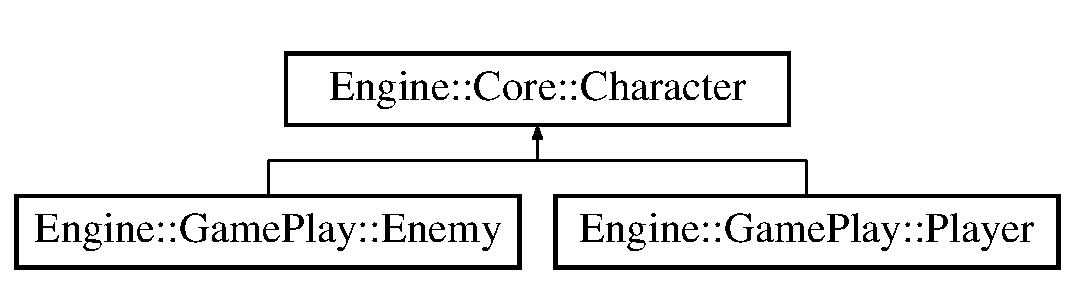
\includegraphics[height=2.000000cm]{class_engine_1_1_core_1_1_character}
\end{center}
\end{figure}
\subsection*{Public Member Functions}
\begin{DoxyCompactItemize}
\item 
\hyperlink{class_engine_1_1_core_1_1_character_a0377de26714b79374d0591ca44c77fd1}{$\sim$\+Character} ()
\item 
Vector2f \hyperlink{class_engine_1_1_core_1_1_character_aea290308ddc56ab784c87f85e6b7f254}{Get\+Position} (void)
\item 
Vector2f \hyperlink{class_engine_1_1_core_1_1_character_a3465481aed27d24909b8e40577f09b10}{Get\+Size} (void)
\item 
void \hyperlink{class_engine_1_1_core_1_1_character_ae25a76e7497eeb6dbd1ad3b72c1ff721}{Draw} (Render\+Window $\ast$Window)
\item 
void \hyperlink{class_engine_1_1_core_1_1_character_a2156c371584ca6a8d2961154f1b49c09}{Take\+Damage} (int Amount)
\item 
\mbox{\Hypertarget{class_engine_1_1_core_1_1_character_ad32924505f5bc7761590ecbfd06e6f09}\label{class_engine_1_1_core_1_1_character_ad32924505f5bc7761590ecbfd06e6f09}} 
bool {\bfseries Check\+Health} (void)
\item 
shared\+\_\+ptr$<$ \hyperlink{class_engine_1_1_core_1_1_game_texture}{Game\+Texture} $>$ \hyperlink{class_engine_1_1_core_1_1_character_afff37c4ff688837f42509f721853bab8}{Get\+Game\+Texure} (void) const
\item 
\mbox{\Hypertarget{class_engine_1_1_core_1_1_character_a45c8ef2c736469a3264ee8733305675c}\label{class_engine_1_1_core_1_1_character_a45c8ef2c736469a3264ee8733305675c}} 
virtual void {\bfseries Update} (Render\+Window $\ast$Window, \hyperlink{class_engine_1_1_core_1_1_map}{Map} M, float dt)=0
\end{DoxyCompactItemize}
\subsection*{Protected Member Functions}
\begin{DoxyCompactItemize}
\item 
\mbox{\Hypertarget{class_engine_1_1_core_1_1_character_ad6e83da3df6620fedbe859022f68727f}\label{class_engine_1_1_core_1_1_character_ad6e83da3df6620fedbe859022f68727f}} 
void {\bfseries Set\+Position} (Vector2f Position)
\end{DoxyCompactItemize}
\subsection*{Protected Attributes}
\begin{DoxyCompactItemize}
\item 
\mbox{\Hypertarget{class_engine_1_1_core_1_1_character_ad98ac89b7c82b587306e83b5aa6acf07}\label{class_engine_1_1_core_1_1_character_ad98ac89b7c82b587306e83b5aa6acf07}} 
float {\bfseries Angle}
\item 
\mbox{\Hypertarget{class_engine_1_1_core_1_1_character_aacac55c620345c41b3eb09f4abbd4318}\label{class_engine_1_1_core_1_1_character_aacac55c620345c41b3eb09f4abbd4318}} 
Vector2f {\bfseries Direction}
\item 
\mbox{\Hypertarget{class_engine_1_1_core_1_1_character_a5f898cc76d7384b27f3105babb9ea27a}\label{class_engine_1_1_core_1_1_character_a5f898cc76d7384b27f3105babb9ea27a}} 
int {\bfseries Health}
\item 
\mbox{\Hypertarget{class_engine_1_1_core_1_1_character_a4b0c92ea505c26b00f1a4873bdf747b2}\label{class_engine_1_1_core_1_1_character_a4b0c92ea505c26b00f1a4873bdf747b2}} 
bool {\bfseries Is\+Alive}
\item 
\mbox{\Hypertarget{class_engine_1_1_core_1_1_character_ab749582f4376b908cdf23d6cc4ac2fe2}\label{class_engine_1_1_core_1_1_character_ab749582f4376b908cdf23d6cc4ac2fe2}} 
Vector2f \hyperlink{class_engine_1_1_core_1_1_character_ab749582f4376b908cdf23d6cc4ac2fe2}{Last\+Good\+Position}
\begin{DoxyCompactList}\small\item\em Saves the last position where the character could move freely. \end{DoxyCompactList}\item 
\mbox{\Hypertarget{class_engine_1_1_core_1_1_character_a289559b0eea38088ed1135ef8cf994dd}\label{class_engine_1_1_core_1_1_character_a289559b0eea38088ed1135ef8cf994dd}} 
shared\+\_\+ptr$<$ \hyperlink{class_engine_1_1_core_1_1_game_texture}{Game\+Texture} $>$ {\bfseries Texture}
\end{DoxyCompactItemize}


\subsection{Constructor \& Destructor Documentation}
\mbox{\Hypertarget{class_engine_1_1_core_1_1_character_a0377de26714b79374d0591ca44c77fd1}\label{class_engine_1_1_core_1_1_character_a0377de26714b79374d0591ca44c77fd1}} 
\index{Engine\+::\+Core\+::\+Character@{Engine\+::\+Core\+::\+Character}!````~Character@{$\sim$\+Character}}
\index{````~Character@{$\sim$\+Character}!Engine\+::\+Core\+::\+Character@{Engine\+::\+Core\+::\+Character}}
\subsubsection{\texorpdfstring{$\sim$\+Character()}{~Character()}}
{\footnotesize\ttfamily Engine\+::\+Core\+::\+Character\+::$\sim$\+Character (\begin{DoxyParamCaption}{ }\end{DoxyParamCaption})}

summary$>$ Gets the position in a sf\+::\+Vector2f. /summary$>$ returns$>$The position as a sf\+::\+Vector2f.

\subsection{Member Function Documentation}
\mbox{\Hypertarget{class_engine_1_1_core_1_1_character_ae25a76e7497eeb6dbd1ad3b72c1ff721}\label{class_engine_1_1_core_1_1_character_ae25a76e7497eeb6dbd1ad3b72c1ff721}} 
\index{Engine\+::\+Core\+::\+Character@{Engine\+::\+Core\+::\+Character}!Draw@{Draw}}
\index{Draw@{Draw}!Engine\+::\+Core\+::\+Character@{Engine\+::\+Core\+::\+Character}}
\subsubsection{\texorpdfstring{Draw()}{Draw()}}
{\footnotesize\ttfamily void Engine\+::\+Core\+::\+Character\+::\+Draw (\begin{DoxyParamCaption}\item[{Render\+Window $\ast$}]{Window }\end{DoxyParamCaption})}

summary$>$ Lowers the amount of health the \hyperlink{class_engine_1_1_core_1_1_character}{Character}. /summary$>$ param name = \char`\"{}\+Amount\char`\"{}$>$The amount of damage which is given to their health (as an integer).\mbox{\Hypertarget{class_engine_1_1_core_1_1_character_afff37c4ff688837f42509f721853bab8}\label{class_engine_1_1_core_1_1_character_afff37c4ff688837f42509f721853bab8}} 
\index{Engine\+::\+Core\+::\+Character@{Engine\+::\+Core\+::\+Character}!Get\+Game\+Texure@{Get\+Game\+Texure}}
\index{Get\+Game\+Texure@{Get\+Game\+Texure}!Engine\+::\+Core\+::\+Character@{Engine\+::\+Core\+::\+Character}}
\subsubsection{\texorpdfstring{Get\+Game\+Texure()}{GetGameTexure()}}
{\footnotesize\ttfamily shared\+\_\+ptr$<$ \hyperlink{class_engine_1_1_core_1_1_game_texture}{Engine\+::\+Core\+::\+Game\+Texture} $>$ Engine\+::\+Core\+::\+Character\+::\+Get\+Game\+Texure (\begin{DoxyParamCaption}\item[{void}]{ }\end{DoxyParamCaption}) const}

summary$>$ Sets the position of the player, within 2D space. /summary$>$ param name = \char`\"{}\+Position\char`\"{}$>$The position to set the Texture in.\mbox{\Hypertarget{class_engine_1_1_core_1_1_character_aea290308ddc56ab784c87f85e6b7f254}\label{class_engine_1_1_core_1_1_character_aea290308ddc56ab784c87f85e6b7f254}} 
\index{Engine\+::\+Core\+::\+Character@{Engine\+::\+Core\+::\+Character}!Get\+Position@{Get\+Position}}
\index{Get\+Position@{Get\+Position}!Engine\+::\+Core\+::\+Character@{Engine\+::\+Core\+::\+Character}}
\subsubsection{\texorpdfstring{Get\+Position()}{GetPosition()}}
{\footnotesize\ttfamily Vector2f Engine\+::\+Core\+::\+Character\+::\+Get\+Position (\begin{DoxyParamCaption}\item[{void}]{ }\end{DoxyParamCaption})}

summary$>$ Gets the size of the S\+F\+ML Texture, as a Vector2f. /summary$>$ returns$>$The size of the Texture.\mbox{\Hypertarget{class_engine_1_1_core_1_1_character_a3465481aed27d24909b8e40577f09b10}\label{class_engine_1_1_core_1_1_character_a3465481aed27d24909b8e40577f09b10}} 
\index{Engine\+::\+Core\+::\+Character@{Engine\+::\+Core\+::\+Character}!Get\+Size@{Get\+Size}}
\index{Get\+Size@{Get\+Size}!Engine\+::\+Core\+::\+Character@{Engine\+::\+Core\+::\+Character}}
\subsubsection{\texorpdfstring{Get\+Size()}{GetSize()}}
{\footnotesize\ttfamily Vector2f Engine\+::\+Core\+::\+Character\+::\+Get\+Size (\begin{DoxyParamCaption}\item[{void}]{ }\end{DoxyParamCaption})}

summary$>$ Renders the \hyperlink{class_engine_1_1_core_1_1_game_texture}{Game\+Texture} to the given Render\+Window. /summary$>$ param name = \char`\"{}\+Window\char`\"{}$>$A pointer to the Render\+Window, which is the target.\mbox{\Hypertarget{class_engine_1_1_core_1_1_character_a2156c371584ca6a8d2961154f1b49c09}\label{class_engine_1_1_core_1_1_character_a2156c371584ca6a8d2961154f1b49c09}} 
\index{Engine\+::\+Core\+::\+Character@{Engine\+::\+Core\+::\+Character}!Take\+Damage@{Take\+Damage}}
\index{Take\+Damage@{Take\+Damage}!Engine\+::\+Core\+::\+Character@{Engine\+::\+Core\+::\+Character}}
\subsubsection{\texorpdfstring{Take\+Damage()}{TakeDamage()}}
{\footnotesize\ttfamily void Engine\+::\+Core\+::\+Character\+::\+Take\+Damage (\begin{DoxyParamCaption}\item[{int}]{Amount }\end{DoxyParamCaption})}

summary$>$ Checks if the health of the current health is above 0. /summary$>$ returns$>$True if the health is above 0, false otherwise.

The documentation for this class was generated from the following files\+:\begin{DoxyCompactItemize}
\item 
Wave\+Game/Character.\+h\item 
Wave\+Game/Character.\+cpp\end{DoxyCompactItemize}

\hypertarget{class_engine_1_1_game_play_1_1_enemy}{}\section{Engine\+:\+:Game\+Play\+:\+:Enemy Class Reference}
\label{class_engine_1_1_game_play_1_1_enemy}\index{Engine\+::\+Game\+Play\+::\+Enemy@{Engine\+::\+Game\+Play\+::\+Enemy}}
Inheritance diagram for Engine\+:\+:Game\+Play\+:\+:Enemy\+:\begin{figure}[H]
\begin{center}
\leavevmode
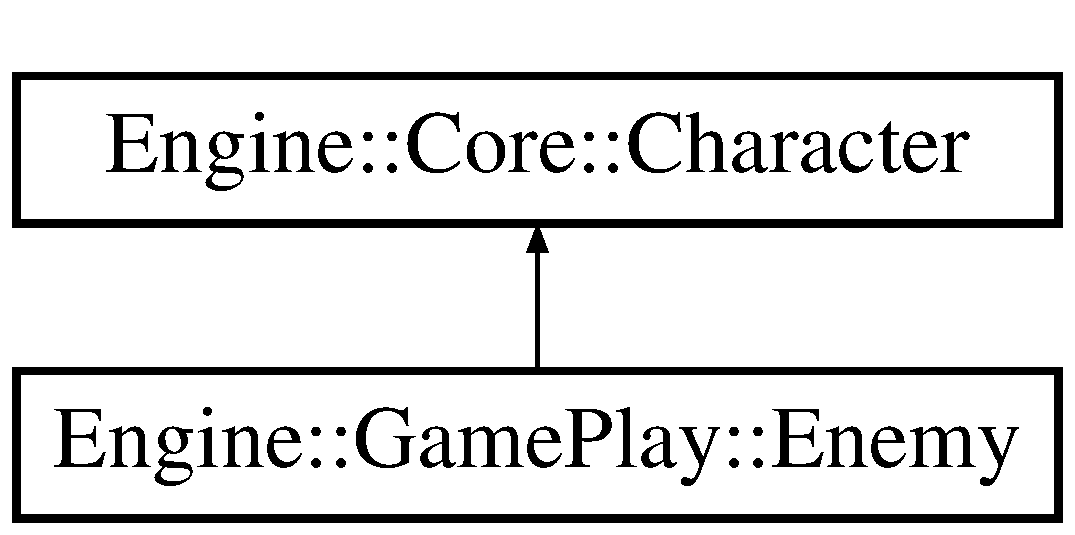
\includegraphics[height=2.000000cm]{class_engine_1_1_game_play_1_1_enemy}
\end{center}
\end{figure}
\subsection*{Public Member Functions}
\begin{DoxyCompactItemize}
\item 
\mbox{\Hypertarget{class_engine_1_1_game_play_1_1_enemy_aecd83da9f05f6d81d512e56f0f16b1d2}\label{class_engine_1_1_game_play_1_1_enemy_aecd83da9f05f6d81d512e56f0f16b1d2}} 
\hyperlink{class_engine_1_1_game_play_1_1_enemy_aecd83da9f05f6d81d512e56f0f16b1d2}{Enemy} (Vector2f Position, Render\+Window $\ast$Window, \hyperlink{class_engine_1_1_game_play_1_1_player}{Player} $\ast$P, float Speed)
\begin{DoxyCompactList}\small\item\em Constructs the enemy object. Loads the Animator from the cache. /summary$>$ param name = \char`\"{}\+Position\char`\"{}$>$The position to set the enemy at.

param name = \char`\"{}\+Window\char`\"{}$>$The window which is being rendered to.

param name = \char`\"{}\+P\char`\"{}$>$The player which is being currently used.

param name = \char`\"{}\+Speed\char`\"{}$>$The speed (in pixels per second) the enemy can move at.\end{DoxyCompactList}\item 
\hyperlink{class_engine_1_1_game_play_1_1_enemy_a4fc3aafb331e8cf852ea31bcc63940ff}{$\sim$\+Enemy} ()
\item 
\mbox{\Hypertarget{class_engine_1_1_game_play_1_1_enemy_a57b75fc882a4315cfda071dbb5c1b5ea}\label{class_engine_1_1_game_play_1_1_enemy_a57b75fc882a4315cfda071dbb5c1b5ea}} 
void {\bfseries Update} (Render\+Window $\ast$Window, \hyperlink{class_engine_1_1_core_1_1_map}{Map} M, float dt) override
\item 
void \hyperlink{class_engine_1_1_game_play_1_1_enemy_a0eec9ea5a61636db10b5f02f9e74189a}{Take\+Damage} (int Amount) override
\end{DoxyCompactItemize}
\subsection*{Additional Inherited Members}


\subsection{Constructor \& Destructor Documentation}
\mbox{\Hypertarget{class_engine_1_1_game_play_1_1_enemy_a4fc3aafb331e8cf852ea31bcc63940ff}\label{class_engine_1_1_game_play_1_1_enemy_a4fc3aafb331e8cf852ea31bcc63940ff}} 
\index{Engine\+::\+Game\+Play\+::\+Enemy@{Engine\+::\+Game\+Play\+::\+Enemy}!````~Enemy@{$\sim$\+Enemy}}
\index{````~Enemy@{$\sim$\+Enemy}!Engine\+::\+Game\+Play\+::\+Enemy@{Engine\+::\+Game\+Play\+::\+Enemy}}
\subsubsection{\texorpdfstring{$\sim$\+Enemy()}{~Enemy()}}
{\footnotesize\ttfamily Engine\+::\+Game\+Play\+::\+Enemy\+::$\sim$\+Enemy (\begin{DoxyParamCaption}{ }\end{DoxyParamCaption})}

summary$>$ Called once per frame, updates the enemy. /summary$>$ param name = \char`\"{}\+Window\char`\"{}$>$A pointer to the Render\+Window which is being used.

param name = \char`\"{}\+M\char`\"{}$>$A copy of the Map for the player for movement.

param name = \char`\"{}dt\char`\"{}$>$Delta time, the time the last frame took.

\subsection{Member Function Documentation}
\mbox{\Hypertarget{class_engine_1_1_game_play_1_1_enemy_a0eec9ea5a61636db10b5f02f9e74189a}\label{class_engine_1_1_game_play_1_1_enemy_a0eec9ea5a61636db10b5f02f9e74189a}} 
\index{Engine\+::\+Game\+Play\+::\+Enemy@{Engine\+::\+Game\+Play\+::\+Enemy}!Take\+Damage@{Take\+Damage}}
\index{Take\+Damage@{Take\+Damage}!Engine\+::\+Game\+Play\+::\+Enemy@{Engine\+::\+Game\+Play\+::\+Enemy}}
\subsubsection{\texorpdfstring{Take\+Damage()}{TakeDamage()}}
{\footnotesize\ttfamily void Engine\+::\+Game\+Play\+::\+Enemy\+::\+Take\+Damage (\begin{DoxyParamCaption}\item[{int}]{Amount }\end{DoxyParamCaption})\hspace{0.3cm}{\ttfamily [override]}, {\ttfamily [virtual]}}

summary$>$ Carries out different functions, depending on the current state. /summary$>$ 

Reimplemented from \hyperlink{class_engine_1_1_core_1_1_character_a2156c371584ca6a8d2961154f1b49c09}{Engine\+::\+Core\+::\+Character}.



The documentation for this class was generated from the following files\+:\begin{DoxyCompactItemize}
\item 
Wave\+Game/Enemy.\+h\item 
Wave\+Game/Enemy.\+cpp\end{DoxyCompactItemize}

\hypertarget{class_engine_1_1_game_play_1_1_enemy_manager}{}\section{Engine\+:\+:Game\+Play\+:\+:Enemy\+Manager Class Reference}
\label{class_engine_1_1_game_play_1_1_enemy_manager}\index{Engine\+::\+Game\+Play\+::\+Enemy\+Manager@{Engine\+::\+Game\+Play\+::\+Enemy\+Manager}}
\subsection*{Public Member Functions}
\begin{DoxyCompactItemize}
\item 
\mbox{\Hypertarget{class_engine_1_1_game_play_1_1_enemy_manager_af20b8cb960acd6a5aabfe6ee5bb9e9e2}\label{class_engine_1_1_game_play_1_1_enemy_manager_af20b8cb960acd6a5aabfe6ee5bb9e9e2}} 
{\bfseries Enemy\+Manager} (Render\+Window $\ast$Window, \hyperlink{class_engine_1_1_game_play_1_1_player}{Player} $\ast$P, mt19937 $\ast$Generator)
\item 
\hyperlink{class_engine_1_1_game_play_1_1_enemy_manager_a503eadcd690205ae495d3761bdfdfcb6}{$\sim$\+Enemy\+Manager} ()
\item 
void \hyperlink{class_engine_1_1_game_play_1_1_enemy_manager_a545df3d86d86905d5db1e4bb8f327137}{Update} (Render\+Window $\ast$Window, \hyperlink{class_engine_1_1_core_1_1_map}{Map} M, float dt)
\item 
void \hyperlink{class_engine_1_1_game_play_1_1_enemy_manager_a8feb401224cac44bec8b2d2c00b0910c}{Draw} (Render\+Window $\ast$Window)
\item 
\mbox{\Hypertarget{class_engine_1_1_game_play_1_1_enemy_manager_afc7a1062c7cf55177a8dd99f8547ec47}\label{class_engine_1_1_game_play_1_1_enemy_manager_afc7a1062c7cf55177a8dd99f8547ec47}} 
vector$<$ \hyperlink{class_engine_1_1_game_play_1_1_enemy}{Enemy} $\ast$ $>$ {\bfseries Get\+Enemies\+In\+Range} (Float\+Rect Bounding\+Box)
\end{DoxyCompactItemize}


\subsection{Constructor \& Destructor Documentation}
\mbox{\Hypertarget{class_engine_1_1_game_play_1_1_enemy_manager_a503eadcd690205ae495d3761bdfdfcb6}\label{class_engine_1_1_game_play_1_1_enemy_manager_a503eadcd690205ae495d3761bdfdfcb6}} 
\index{Engine\+::\+Game\+Play\+::\+Enemy\+Manager@{Engine\+::\+Game\+Play\+::\+Enemy\+Manager}!````~Enemy\+Manager@{$\sim$\+Enemy\+Manager}}
\index{````~Enemy\+Manager@{$\sim$\+Enemy\+Manager}!Engine\+::\+Game\+Play\+::\+Enemy\+Manager@{Engine\+::\+Game\+Play\+::\+Enemy\+Manager}}
\subsubsection{\texorpdfstring{$\sim$\+Enemy\+Manager()}{~EnemyManager()}}
{\footnotesize\ttfamily Engine\+::\+Game\+Play\+::\+Enemy\+Manager\+::$\sim$\+Enemy\+Manager (\begin{DoxyParamCaption}{ }\end{DoxyParamCaption})}

summary$>$ Called once per frame. Handles the states of the match. Updates each enemy, when they\textquotesingle{}re all dead the state is changed to Interval. Then the game deletes the pointers to the dead enemies, then a timer is ran. Once the timer is up, the state is switched to New\+Match. This spawns in the new enemies, the amount is D\+E\+F\+A\+U\+L\+T\+\_\+\+E\+N\+E\+M\+Y\+\_\+\+C\+O\+U\+NT + Current\+Wave. Once they\textquotesingle{}re all spawned the state is switched to In\+Match. /summary$>$ param name = \char`\"{}\+Window\char`\"{}$>$The window used to draw to.

param name = \char`\"{}\+M\char`\"{}$>$The map which is being played.

param name = \char`\"{}dt\char`\"{}$>$Deltatime.

\subsection{Member Function Documentation}
\mbox{\Hypertarget{class_engine_1_1_game_play_1_1_enemy_manager_a8feb401224cac44bec8b2d2c00b0910c}\label{class_engine_1_1_game_play_1_1_enemy_manager_a8feb401224cac44bec8b2d2c00b0910c}} 
\index{Engine\+::\+Game\+Play\+::\+Enemy\+Manager@{Engine\+::\+Game\+Play\+::\+Enemy\+Manager}!Draw@{Draw}}
\index{Draw@{Draw}!Engine\+::\+Game\+Play\+::\+Enemy\+Manager@{Engine\+::\+Game\+Play\+::\+Enemy\+Manager}}
\subsubsection{\texorpdfstring{Draw()}{Draw()}}
{\footnotesize\ttfamily void Engine\+::\+Game\+Play\+::\+Enemy\+Manager\+::\+Draw (\begin{DoxyParamCaption}\item[{Render\+Window $\ast$}]{Window }\end{DoxyParamCaption})}

summary$>$ Gets enemies within a bounding box. /summary$>$ param name = \char`\"{}\+Bounding\+Box\char`\"{}$>$The bounding box to test if the enemies within.

returns$>$A vector of pointers to enemies.\mbox{\Hypertarget{class_engine_1_1_game_play_1_1_enemy_manager_a545df3d86d86905d5db1e4bb8f327137}\label{class_engine_1_1_game_play_1_1_enemy_manager_a545df3d86d86905d5db1e4bb8f327137}} 
\index{Engine\+::\+Game\+Play\+::\+Enemy\+Manager@{Engine\+::\+Game\+Play\+::\+Enemy\+Manager}!Update@{Update}}
\index{Update@{Update}!Engine\+::\+Game\+Play\+::\+Enemy\+Manager@{Engine\+::\+Game\+Play\+::\+Enemy\+Manager}}
\subsubsection{\texorpdfstring{Update()}{Update()}}
{\footnotesize\ttfamily void Engine\+::\+Game\+Play\+::\+Enemy\+Manager\+::\+Update (\begin{DoxyParamCaption}\item[{Render\+Window $\ast$}]{Window,  }\item[{\hyperlink{class_engine_1_1_core_1_1_map}{Map}}]{M,  }\item[{float}]{dt }\end{DoxyParamCaption})}

summary$>$ Draws the text displaying the round information, then the enemies. /summary$>$ param name = \char`\"{}\+Window\char`\"{}$>$The Render\+Window to draw to.

The documentation for this class was generated from the following files\+:\begin{DoxyCompactItemize}
\item 
Wave\+Game/Enemy\+Manager.\+h\item 
Wave\+Game/Enemy\+Manager.\+cpp\end{DoxyCompactItemize}

\hypertarget{class_fixed_size_allocator}{}\section{Fixed\+Size\+Allocator$<$ U\+S\+E\+R\+\_\+\+T\+Y\+PE $>$ Class Template Reference}
\label{class_fixed_size_allocator}\index{Fixed\+Size\+Allocator$<$ U\+S\+E\+R\+\_\+\+T\+Y\+P\+E $>$@{Fixed\+Size\+Allocator$<$ U\+S\+E\+R\+\_\+\+T\+Y\+P\+E $>$}}
\subsection*{Classes}
\begin{DoxyCompactItemize}
\item 
struct \hyperlink{struct_fixed_size_allocator_1_1_f_s_a___e_l_e_m_e_n_t}{F\+S\+A\+\_\+\+E\+L\+E\+M\+E\+NT}
\end{DoxyCompactItemize}
\subsection*{Public Types}
\begin{DoxyCompactItemize}
\item 
\mbox{\Hypertarget{class_fixed_size_allocator_ac1babd155fdc91afbf6f482b72159bed}\label{class_fixed_size_allocator_ac1babd155fdc91afbf6f482b72159bed}} 
enum \{ {\bfseries F\+S\+A\+\_\+\+D\+E\+F\+A\+U\+L\+T\+\_\+\+S\+I\+ZE} = 100
 \}
\end{DoxyCompactItemize}
\subsection*{Public Member Functions}
\begin{DoxyCompactItemize}
\item 
\mbox{\Hypertarget{class_fixed_size_allocator_ae5c456344d0c741b01c9441573159586}\label{class_fixed_size_allocator_ae5c456344d0c741b01c9441573159586}} 
{\bfseries Fixed\+Size\+Allocator} (unsigned int Max\+Elements=F\+S\+A\+\_\+\+D\+E\+F\+A\+U\+L\+T\+\_\+\+S\+I\+ZE)
\item 
\mbox{\Hypertarget{class_fixed_size_allocator_ac48055f3218de0c25caa71312ddd71a0}\label{class_fixed_size_allocator_ac48055f3218de0c25caa71312ddd71a0}} 
U\+S\+E\+R\+\_\+\+T\+Y\+PE $\ast$ {\bfseries alloc} ()
\item 
\mbox{\Hypertarget{class_fixed_size_allocator_a2c8cfe0b5c46c9e11baf09a86f369b58}\label{class_fixed_size_allocator_a2c8cfe0b5c46c9e11baf09a86f369b58}} 
void {\bfseries free} (U\+S\+E\+R\+\_\+\+T\+Y\+PE $\ast$user\+\_\+data)
\item 
\mbox{\Hypertarget{class_fixed_size_allocator_afec18245a3195a6aaad728f371abc4a9}\label{class_fixed_size_allocator_afec18245a3195a6aaad728f371abc4a9}} 
void {\bfseries Debug} ()
\item 
\mbox{\Hypertarget{class_fixed_size_allocator_a483c3ae6aa4869a622f018a1bb7de4b7}\label{class_fixed_size_allocator_a483c3ae6aa4869a622f018a1bb7de4b7}} 
U\+S\+E\+R\+\_\+\+T\+Y\+PE $\ast$ {\bfseries Get\+First} ()
\item 
\mbox{\Hypertarget{class_fixed_size_allocator_abc6a00b10f0853c011b7b0105293165a}\label{class_fixed_size_allocator_abc6a00b10f0853c011b7b0105293165a}} 
U\+S\+E\+R\+\_\+\+T\+Y\+PE $\ast$ {\bfseries Get\+Next} (U\+S\+E\+R\+\_\+\+T\+Y\+PE $\ast$node)
\end{DoxyCompactItemize}


The documentation for this class was generated from the following file\+:\begin{DoxyCompactItemize}
\item 
Wave\+Game/fsa.\+h\end{DoxyCompactItemize}

\hypertarget{struct_fixed_size_allocator_1_1_f_s_a___e_l_e_m_e_n_t}{}\section{Fixed\+Size\+Allocator$<$ U\+S\+E\+R\+\_\+\+T\+Y\+PE $>$\+:\+:F\+S\+A\+\_\+\+E\+L\+E\+M\+E\+NT Struct Reference}
\label{struct_fixed_size_allocator_1_1_f_s_a___e_l_e_m_e_n_t}\index{Fixed\+Size\+Allocator$<$ U\+S\+E\+R\+\_\+\+T\+Y\+P\+E $>$\+::\+F\+S\+A\+\_\+\+E\+L\+E\+M\+E\+NT@{Fixed\+Size\+Allocator$<$ U\+S\+E\+R\+\_\+\+T\+Y\+P\+E $>$\+::\+F\+S\+A\+\_\+\+E\+L\+E\+M\+E\+NT}}
\subsection*{Public Attributes}
\begin{DoxyCompactItemize}
\item 
\mbox{\Hypertarget{struct_fixed_size_allocator_1_1_f_s_a___e_l_e_m_e_n_t_ab03c9e3fd88ea983170e40dd23a70473}\label{struct_fixed_size_allocator_1_1_f_s_a___e_l_e_m_e_n_t_ab03c9e3fd88ea983170e40dd23a70473}} 
U\+S\+E\+R\+\_\+\+T\+Y\+PE {\bfseries User\+Type}
\item 
\mbox{\Hypertarget{struct_fixed_size_allocator_1_1_f_s_a___e_l_e_m_e_n_t_a2392c4eaf0fe0f15451076d9fc9348ea}\label{struct_fixed_size_allocator_1_1_f_s_a___e_l_e_m_e_n_t_a2392c4eaf0fe0f15451076d9fc9348ea}} 
\hyperlink{struct_fixed_size_allocator_1_1_f_s_a___e_l_e_m_e_n_t}{F\+S\+A\+\_\+\+E\+L\+E\+M\+E\+NT} $\ast$ {\bfseries p\+Prev}
\item 
\mbox{\Hypertarget{struct_fixed_size_allocator_1_1_f_s_a___e_l_e_m_e_n_t_a286ad3e87228466107eef29e6e5a7d81}\label{struct_fixed_size_allocator_1_1_f_s_a___e_l_e_m_e_n_t_a286ad3e87228466107eef29e6e5a7d81}} 
\hyperlink{struct_fixed_size_allocator_1_1_f_s_a___e_l_e_m_e_n_t}{F\+S\+A\+\_\+\+E\+L\+E\+M\+E\+NT} $\ast$ {\bfseries p\+Next}
\end{DoxyCompactItemize}


The documentation for this struct was generated from the following file\+:\begin{DoxyCompactItemize}
\item 
Wave\+Game/fsa.\+h\end{DoxyCompactItemize}

\hypertarget{class_engine_1_1_core_1_1_game_texture}{}\section{Engine\+:\+:Core\+:\+:Game\+Texture Class Reference}
\label{class_engine_1_1_core_1_1_game_texture}\index{Engine\+::\+Core\+::\+Game\+Texture@{Engine\+::\+Core\+::\+Game\+Texture}}


Wraps around the S\+F\+ML texture and puts both sf\+::\+Texture and sf\+::\+Sprite into one object. /summary$>$  




{\ttfamily \#include $<$Game\+Texture.\+h$>$}

\subsection*{Public Member Functions}
\begin{DoxyCompactItemize}
\item 
\mbox{\Hypertarget{class_engine_1_1_core_1_1_game_texture_ae9eb069dd4a60ad5af6e19ca35432ea2}\label{class_engine_1_1_core_1_1_game_texture_ae9eb069dd4a60ad5af6e19ca35432ea2}} 
{\bfseries Game\+Texture} (const string \&Path)
\item 
\mbox{\Hypertarget{class_engine_1_1_core_1_1_game_texture_a5d6076b052118c2212b103cbdf3ea836}\label{class_engine_1_1_core_1_1_game_texture_a5d6076b052118c2212b103cbdf3ea836}} 
{\bfseries Game\+Texture} (const \hyperlink{class_engine_1_1_core_1_1_game_texture}{Game\+Texture} \&Tex)
\item 
\mbox{\Hypertarget{class_engine_1_1_core_1_1_game_texture_aac115d213538922ab88a656b6780b6b3}\label{class_engine_1_1_core_1_1_game_texture_aac115d213538922ab88a656b6780b6b3}} 
{\bfseries Game\+Texture} (Texture Tex)
\item 
\hyperlink{class_engine_1_1_core_1_1_game_texture_a37c2ee2ebfdfc3301b6070d2df10d59a}{$\sim$\+Game\+Texture} ()
\item 
Texture \hyperlink{class_engine_1_1_core_1_1_game_texture_a07e51ed155d0c9b24197444b473cbf19}{Get\+S\+F\+M\+L\+Texture} (void) const
\item 
shared\+\_\+ptr$<$ Sprite $>$ \hyperlink{class_engine_1_1_core_1_1_game_texture_aec2df0beae7b8693160e20c1fd3588ac}{Get\+S\+F\+M\+L\+Sprite} (void)
\item 
void \hyperlink{class_engine_1_1_core_1_1_game_texture_ae1f94e0f1b86e99ed4508ccdda4872d6}{Set\+Position} (const Vector2f \&Position)
\item 
void \hyperlink{class_engine_1_1_core_1_1_game_texture_a5ed78714df6128f09c35c25e2271dc05}{Set\+Rotation} (float Angle)
\item 
void \hyperlink{class_engine_1_1_core_1_1_game_texture_aa01df5d689abf48b1d442da329485eeb}{Set\+Origin} (const Vector2f \&Position)
\item 
void \hyperlink{class_engine_1_1_core_1_1_game_texture_af0169ac026c5b15cb3195d1199b13d33}{Move} (const Vector2f \&Offset)
\item 
\mbox{\Hypertarget{class_engine_1_1_core_1_1_game_texture_a103ed3e78d64382d3e82b5fca05ceccd}\label{class_engine_1_1_core_1_1_game_texture_a103ed3e78d64382d3e82b5fca05ceccd}} 
void {\bfseries Draw} (shared\+\_\+ptr$<$ Render\+Window $>$ Render\+Window)
\end{DoxyCompactItemize}


\subsection{Detailed Description}
Wraps around the S\+F\+ML texture and puts both sf\+::\+Texture and sf\+::\+Sprite into one object. /summary$>$ 

\subsection{Constructor \& Destructor Documentation}
\mbox{\Hypertarget{class_engine_1_1_core_1_1_game_texture_a37c2ee2ebfdfc3301b6070d2df10d59a}\label{class_engine_1_1_core_1_1_game_texture_a37c2ee2ebfdfc3301b6070d2df10d59a}} 
\index{Engine\+::\+Core\+::\+Game\+Texture@{Engine\+::\+Core\+::\+Game\+Texture}!````~Game\+Texture@{$\sim$\+Game\+Texture}}
\index{````~Game\+Texture@{$\sim$\+Game\+Texture}!Engine\+::\+Core\+::\+Game\+Texture@{Engine\+::\+Core\+::\+Game\+Texture}}
\subsubsection{\texorpdfstring{$\sim$\+Game\+Texture()}{~GameTexture()}}
{\footnotesize\ttfamily Engine\+::\+Core\+::\+Game\+Texture\+::$\sim$\+Game\+Texture (\begin{DoxyParamCaption}{ }\end{DoxyParamCaption})}

summary$>$ Gets the sf\+::\+Texture which is used by the object. /summary$>$ returns$>$The sf\+::\+Texture used.

\subsection{Member Function Documentation}
\mbox{\Hypertarget{class_engine_1_1_core_1_1_game_texture_aec2df0beae7b8693160e20c1fd3588ac}\label{class_engine_1_1_core_1_1_game_texture_aec2df0beae7b8693160e20c1fd3588ac}} 
\index{Engine\+::\+Core\+::\+Game\+Texture@{Engine\+::\+Core\+::\+Game\+Texture}!Get\+S\+F\+M\+L\+Sprite@{Get\+S\+F\+M\+L\+Sprite}}
\index{Get\+S\+F\+M\+L\+Sprite@{Get\+S\+F\+M\+L\+Sprite}!Engine\+::\+Core\+::\+Game\+Texture@{Engine\+::\+Core\+::\+Game\+Texture}}
\subsubsection{\texorpdfstring{Get\+S\+F\+M\+L\+Sprite()}{GetSFMLSprite()}}
{\footnotesize\ttfamily shared\+\_\+ptr$<$ Sprite $>$ Engine\+::\+Core\+::\+Game\+Texture\+::\+Get\+S\+F\+M\+L\+Sprite (\begin{DoxyParamCaption}\item[{void}]{ }\end{DoxyParamCaption})}

summary$>$ Sets the position of the sprite, in 2D space. /summary$>$ param name = \char`\"{}\+Position\char`\"{}$>$The position to set the \mbox{\Hypertarget{class_engine_1_1_core_1_1_game_texture_a07e51ed155d0c9b24197444b473cbf19}\label{class_engine_1_1_core_1_1_game_texture_a07e51ed155d0c9b24197444b473cbf19}} 
\index{Engine\+::\+Core\+::\+Game\+Texture@{Engine\+::\+Core\+::\+Game\+Texture}!Get\+S\+F\+M\+L\+Texture@{Get\+S\+F\+M\+L\+Texture}}
\index{Get\+S\+F\+M\+L\+Texture@{Get\+S\+F\+M\+L\+Texture}!Engine\+::\+Core\+::\+Game\+Texture@{Engine\+::\+Core\+::\+Game\+Texture}}
\subsubsection{\texorpdfstring{Get\+S\+F\+M\+L\+Texture()}{GetSFMLTexture()}}
{\footnotesize\ttfamily Texture Engine\+::\+Core\+::\+Game\+Texture\+::\+Get\+S\+F\+M\+L\+Texture (\begin{DoxyParamCaption}\item[{void}]{ }\end{DoxyParamCaption}) const}

summary$>$ Gets the sf\+::\+Sprite used by the object. /summary$>$ returns$>$A shared\+\_\+ptr to the sf\+::sprite.\mbox{\Hypertarget{class_engine_1_1_core_1_1_game_texture_af0169ac026c5b15cb3195d1199b13d33}\label{class_engine_1_1_core_1_1_game_texture_af0169ac026c5b15cb3195d1199b13d33}} 
\index{Engine\+::\+Core\+::\+Game\+Texture@{Engine\+::\+Core\+::\+Game\+Texture}!Move@{Move}}
\index{Move@{Move}!Engine\+::\+Core\+::\+Game\+Texture@{Engine\+::\+Core\+::\+Game\+Texture}}
\subsubsection{\texorpdfstring{Move()}{Move()}}
{\footnotesize\ttfamily void Engine\+::\+Core\+::\+Game\+Texture\+::\+Move (\begin{DoxyParamCaption}\item[{const Vector2f \&}]{Offset }\end{DoxyParamCaption})}

summary$>$ Renders the texture to the screen. /summary$>$ param name = \char`\"{}\+Render\+Window\char`\"{}$>$The window to draw to.

exception cref = \char`\"{}std\+::runtime\+\_\+error\char`\"{}$>$Throws if Render\+Window is a nullptr.\mbox{\Hypertarget{class_engine_1_1_core_1_1_game_texture_aa01df5d689abf48b1d442da329485eeb}\label{class_engine_1_1_core_1_1_game_texture_aa01df5d689abf48b1d442da329485eeb}} 
\index{Engine\+::\+Core\+::\+Game\+Texture@{Engine\+::\+Core\+::\+Game\+Texture}!Set\+Origin@{Set\+Origin}}
\index{Set\+Origin@{Set\+Origin}!Engine\+::\+Core\+::\+Game\+Texture@{Engine\+::\+Core\+::\+Game\+Texture}}
\subsubsection{\texorpdfstring{Set\+Origin()}{SetOrigin()}}
{\footnotesize\ttfamily void Engine\+::\+Core\+::\+Game\+Texture\+::\+Set\+Origin (\begin{DoxyParamCaption}\item[{const Vector2f \&}]{Position }\end{DoxyParamCaption})}

summary$>$ Moves the texture a given amount of pixels across the screen. /summary$>$ param name = \char`\"{}\+Offset\char`\"{}$>$The amount of pixels to move the texture by from its current position.\mbox{\Hypertarget{class_engine_1_1_core_1_1_game_texture_ae1f94e0f1b86e99ed4508ccdda4872d6}\label{class_engine_1_1_core_1_1_game_texture_ae1f94e0f1b86e99ed4508ccdda4872d6}} 
\index{Engine\+::\+Core\+::\+Game\+Texture@{Engine\+::\+Core\+::\+Game\+Texture}!Set\+Position@{Set\+Position}}
\index{Set\+Position@{Set\+Position}!Engine\+::\+Core\+::\+Game\+Texture@{Engine\+::\+Core\+::\+Game\+Texture}}
\subsubsection{\texorpdfstring{Set\+Position()}{SetPosition()}}
{\footnotesize\ttfamily void Engine\+::\+Core\+::\+Game\+Texture\+::\+Set\+Position (\begin{DoxyParamCaption}\item[{const Vector2f \&}]{Position }\end{DoxyParamCaption})}

summary$>$ Sets the rotation of the texture. /summary$>$ param name = \char`\"{}\+Angle\char`\"{}$>$The angle to set the player to.\mbox{\Hypertarget{class_engine_1_1_core_1_1_game_texture_a5ed78714df6128f09c35c25e2271dc05}\label{class_engine_1_1_core_1_1_game_texture_a5ed78714df6128f09c35c25e2271dc05}} 
\index{Engine\+::\+Core\+::\+Game\+Texture@{Engine\+::\+Core\+::\+Game\+Texture}!Set\+Rotation@{Set\+Rotation}}
\index{Set\+Rotation@{Set\+Rotation}!Engine\+::\+Core\+::\+Game\+Texture@{Engine\+::\+Core\+::\+Game\+Texture}}
\subsubsection{\texorpdfstring{Set\+Rotation()}{SetRotation()}}
{\footnotesize\ttfamily void Engine\+::\+Core\+::\+Game\+Texture\+::\+Set\+Rotation (\begin{DoxyParamCaption}\item[{float}]{Angle }\end{DoxyParamCaption})}

summary$>$ Sets the origin for rotating the texutre. /summary$>$ param name = \char`\"{}\+Position\char`\"{}$>$The position, relative to the sprite, to rotate the texture by.

The documentation for this class was generated from the following files\+:\begin{DoxyCompactItemize}
\item 
Wave\+Game/Game\+Texture.\+h\item 
Wave\+Game/Game\+Texture.\+cpp\end{DoxyCompactItemize}

\hypertarget{class_game_time}{}\section{Game\+Time Class Reference}
\label{class_game_time}\index{Game\+Time@{Game\+Time}}


A class detailing information about the time which frames take to complete.  




{\ttfamily \#include $<$Game\+Time.\+h$>$}

\subsection*{Static Public Member Functions}
\begin{DoxyCompactItemize}
\item 
static void \hyperlink{class_game_time_a1f310e807ddb53d1a1278c4a0a2785ed}{Init} ()
\begin{DoxyCompactList}\small\item\em Initalises the game timer. \end{DoxyCompactList}\item 
static int \hyperlink{class_game_time_a2108b642689adae6830b9e8c9c04b535}{Delta\+Time} ()
\item 
\mbox{\Hypertarget{class_game_time_a2d9927ce7e6cf48da7e8b48a4f1b917f}\label{class_game_time_a2d9927ce7e6cf48da7e8b48a4f1b917f}} 
static void {\bfseries Update} ()
\end{DoxyCompactItemize}


\subsection{Detailed Description}
A class detailing information about the time which frames take to complete. 



\subsection{Member Function Documentation}
\mbox{\Hypertarget{class_game_time_a2108b642689adae6830b9e8c9c04b535}\label{class_game_time_a2108b642689adae6830b9e8c9c04b535}} 
\index{Game\+Time@{Game\+Time}!Delta\+Time@{Delta\+Time}}
\index{Delta\+Time@{Delta\+Time}!Game\+Time@{Game\+Time}}
\subsubsection{\texorpdfstring{Delta\+Time()}{DeltaTime()}}
{\footnotesize\ttfamily int Game\+Time\+::\+Delta\+Time (\begin{DoxyParamCaption}{ }\end{DoxyParamCaption})\hspace{0.3cm}{\ttfamily [static]}}





\mbox{\Hypertarget{class_game_time_a1f310e807ddb53d1a1278c4a0a2785ed}\label{class_game_time_a1f310e807ddb53d1a1278c4a0a2785ed}} 
\index{Game\+Time@{Game\+Time}!Init@{Init}}
\index{Init@{Init}!Game\+Time@{Game\+Time}}
\subsubsection{\texorpdfstring{Init()}{Init()}}
{\footnotesize\ttfamily void Game\+Time\+::\+Init (\begin{DoxyParamCaption}{ }\end{DoxyParamCaption})\hspace{0.3cm}{\ttfamily [static]}}



Initalises the game timer. 



The documentation for this class was generated from the following files\+:\begin{DoxyCompactItemize}
\item 
Wave\+Game/Game\+Time.\+h\item 
Wave\+Game/Game\+Time.\+cpp\end{DoxyCompactItemize}

\hypertarget{class_a_star_search_1_1_heap_compare__f}{}\section{A\+Star\+Search$<$ User\+State $>$\+:\+:Heap\+Compare\+\_\+f Class Reference}
\label{class_a_star_search_1_1_heap_compare__f}\index{A\+Star\+Search$<$ User\+State $>$\+::\+Heap\+Compare\+\_\+f@{A\+Star\+Search$<$ User\+State $>$\+::\+Heap\+Compare\+\_\+f}}
\subsection*{Public Member Functions}
\begin{DoxyCompactItemize}
\item 
\mbox{\Hypertarget{class_a_star_search_1_1_heap_compare__f_a470f1b699b682dc8c4b4b490372bd8ff}\label{class_a_star_search_1_1_heap_compare__f_a470f1b699b682dc8c4b4b490372bd8ff}} 
bool {\bfseries operator()} (const \hyperlink{class_a_star_search_1_1_node}{Node} $\ast$x, const \hyperlink{class_a_star_search_1_1_node}{Node} $\ast$y) const
\end{DoxyCompactItemize}


The documentation for this class was generated from the following file\+:\begin{DoxyCompactItemize}
\item 
Wave\+Game/stlastar.\+h\end{DoxyCompactItemize}

\hypertarget{class_engine_1_1_core_1_1_map}{}\section{Engine\+:\+:Core\+:\+:Map Class Reference}
\label{class_engine_1_1_core_1_1_map}\index{Engine\+::\+Core\+::\+Map@{Engine\+::\+Core\+::\+Map}}
\subsection*{Public Member Functions}
\begin{DoxyCompactItemize}
\item 
\hyperlink{class_engine_1_1_core_1_1_map_a211f38a71b97179bbbd153442225a273}{$\sim$\+Map} ()
\item 
void \hyperlink{class_engine_1_1_core_1_1_map_aa81a28822b49c3c7750f0444a189ed8c}{Add\+Background} (string ID)
\item 
void \hyperlink{class_engine_1_1_core_1_1_map_aad4517115b5d8713aed2f67338cd7259}{Add\+Prop} (string ID, Vector2f Position)
\item 
vector$<$ shared\+\_\+ptr$<$ \hyperlink{class_engine_1_1_core_1_1_game_texture}{Game\+Texture} $>$ $>$ \hyperlink{class_engine_1_1_core_1_1_map_afafd62cdfe87b27796d0900e76aa09ea}{Get\+Props} (void)
\item 
void \hyperlink{class_engine_1_1_core_1_1_map_aeb4eabaf8cbde4e584836daa646c0521}{Draw\+Background} (shared\+\_\+ptr$<$ Render\+Window $>$ Window)
\item 
\mbox{\Hypertarget{class_engine_1_1_core_1_1_map_a2e6a7e15ecd79f449fe6326768069953}\label{class_engine_1_1_core_1_1_map_a2e6a7e15ecd79f449fe6326768069953}} 
void {\bfseries Draw\+Props} (shared\+\_\+ptr$<$ Render\+Window $>$ Window)
\end{DoxyCompactItemize}


\subsection{Constructor \& Destructor Documentation}
\mbox{\Hypertarget{class_engine_1_1_core_1_1_map_a211f38a71b97179bbbd153442225a273}\label{class_engine_1_1_core_1_1_map_a211f38a71b97179bbbd153442225a273}} 
\index{Engine\+::\+Core\+::\+Map@{Engine\+::\+Core\+::\+Map}!````~Map@{$\sim$\+Map}}
\index{````~Map@{$\sim$\+Map}!Engine\+::\+Core\+::\+Map@{Engine\+::\+Core\+::\+Map}}
\subsubsection{\texorpdfstring{$\sim$\+Map()}{~Map()}}
{\footnotesize\ttfamily Engine\+::\+Core\+::\+Map\+::$\sim$\+Map (\begin{DoxyParamCaption}{ }\end{DoxyParamCaption})}

summary$>$ Sets what the background texture is for the map. /summary$>$ param name = \char`\"{}\+I\+D\char`\"{}$>$A string which is the ID of the texture for the background.

\subsection{Member Function Documentation}
\mbox{\Hypertarget{class_engine_1_1_core_1_1_map_aa81a28822b49c3c7750f0444a189ed8c}\label{class_engine_1_1_core_1_1_map_aa81a28822b49c3c7750f0444a189ed8c}} 
\index{Engine\+::\+Core\+::\+Map@{Engine\+::\+Core\+::\+Map}!Add\+Background@{Add\+Background}}
\index{Add\+Background@{Add\+Background}!Engine\+::\+Core\+::\+Map@{Engine\+::\+Core\+::\+Map}}
\subsubsection{\texorpdfstring{Add\+Background()}{AddBackground()}}
{\footnotesize\ttfamily void Engine\+::\+Core\+::\+Map\+::\+Add\+Background (\begin{DoxyParamCaption}\item[{string}]{ID }\end{DoxyParamCaption})}

summary$>$ Adds a prop to the Props vector, so they can be drawn. /summary$>$ param name = \char`\"{}\+I\+D\char`\"{}$>$A string which is the ID for the texture.

param name = \char`\"{}\+Position\char`\"{}$>$A Vector2f which contains the on screen position for the prop.\mbox{\Hypertarget{class_engine_1_1_core_1_1_map_aad4517115b5d8713aed2f67338cd7259}\label{class_engine_1_1_core_1_1_map_aad4517115b5d8713aed2f67338cd7259}} 
\index{Engine\+::\+Core\+::\+Map@{Engine\+::\+Core\+::\+Map}!Add\+Prop@{Add\+Prop}}
\index{Add\+Prop@{Add\+Prop}!Engine\+::\+Core\+::\+Map@{Engine\+::\+Core\+::\+Map}}
\subsubsection{\texorpdfstring{Add\+Prop()}{AddProp()}}
{\footnotesize\ttfamily void Engine\+::\+Core\+::\+Map\+::\+Add\+Prop (\begin{DoxyParamCaption}\item[{string}]{ID,  }\item[{Vector2f}]{Position }\end{DoxyParamCaption})}

summary$>$ Gets all props which are loaded into the map. /summary$>$ returns$>$The props which are loaded in the map.\mbox{\Hypertarget{class_engine_1_1_core_1_1_map_aeb4eabaf8cbde4e584836daa646c0521}\label{class_engine_1_1_core_1_1_map_aeb4eabaf8cbde4e584836daa646c0521}} 
\index{Engine\+::\+Core\+::\+Map@{Engine\+::\+Core\+::\+Map}!Draw\+Background@{Draw\+Background}}
\index{Draw\+Background@{Draw\+Background}!Engine\+::\+Core\+::\+Map@{Engine\+::\+Core\+::\+Map}}
\subsubsection{\texorpdfstring{Draw\+Background()}{DrawBackground()}}
{\footnotesize\ttfamily void Engine\+::\+Core\+::\+Map\+::\+Draw\+Background (\begin{DoxyParamCaption}\item[{shared\+\_\+ptr$<$ Render\+Window $>$}]{Window }\end{DoxyParamCaption})}

summary$>$ Draws the prop to the screen. /summary$>$ param name = \char`\"{}\+Window\char`\"{}$>$A pointer to the Render\+Window is being drawn to.\mbox{\Hypertarget{class_engine_1_1_core_1_1_map_afafd62cdfe87b27796d0900e76aa09ea}\label{class_engine_1_1_core_1_1_map_afafd62cdfe87b27796d0900e76aa09ea}} 
\index{Engine\+::\+Core\+::\+Map@{Engine\+::\+Core\+::\+Map}!Get\+Props@{Get\+Props}}
\index{Get\+Props@{Get\+Props}!Engine\+::\+Core\+::\+Map@{Engine\+::\+Core\+::\+Map}}
\subsubsection{\texorpdfstring{Get\+Props()}{GetProps()}}
{\footnotesize\ttfamily vector$<$ shared\+\_\+ptr$<$ \hyperlink{class_engine_1_1_core_1_1_game_texture}{Engine\+::\+Core\+::\+Game\+Texture} $>$ $>$ Engine\+::\+Core\+::\+Map\+::\+Get\+Props (\begin{DoxyParamCaption}\item[{void}]{ }\end{DoxyParamCaption})}

summary$>$ Draws the background. The background is the first thing which should be drawn. This ensures that the props, player and enemies are on top of it. /summary$>$ param name = \char`\"{}\+Window\char`\"{}$>$A pointer to the Render\+Window is being drawn to.

The documentation for this class was generated from the following files\+:\begin{DoxyCompactItemize}
\item 
Wave\+Game/Map.\+h\item 
Wave\+Game/Map.\+cpp\end{DoxyCompactItemize}

\hypertarget{class_engine_1_1_core_1_1_map_loader}{}\section{Engine\+:\+:Core\+:\+:Map\+Loader Class Reference}
\label{class_engine_1_1_core_1_1_map_loader}\index{Engine\+::\+Core\+::\+Map\+Loader@{Engine\+::\+Core\+::\+Map\+Loader}}
\subsection*{Static Public Member Functions}
\begin{DoxyCompactItemize}
\item 
static \hyperlink{class_engine_1_1_core_1_1_map}{Map} \hyperlink{class_engine_1_1_core_1_1_map_loader_af8d42cc4deb8d177be42b2e9b1277840}{Load} (string Path)
\end{DoxyCompactItemize}


\subsection{Member Function Documentation}
\mbox{\Hypertarget{class_engine_1_1_core_1_1_map_loader_af8d42cc4deb8d177be42b2e9b1277840}\label{class_engine_1_1_core_1_1_map_loader_af8d42cc4deb8d177be42b2e9b1277840}} 
\index{Engine\+::\+Core\+::\+Map\+Loader@{Engine\+::\+Core\+::\+Map\+Loader}!Load@{Load}}
\index{Load@{Load}!Engine\+::\+Core\+::\+Map\+Loader@{Engine\+::\+Core\+::\+Map\+Loader}}
\subsubsection{\texorpdfstring{Load()}{Load()}}
{\footnotesize\ttfamily \hyperlink{class_engine_1_1_core_1_1_map}{Engine\+::\+Core\+::\+Map} Engine\+::\+Core\+::\+Map\+Loader\+::\+Load (\begin{DoxyParamCaption}\item[{string}]{Path }\end{DoxyParamCaption})\hspace{0.3cm}{\ttfamily [static]}}

Load in all of the props into the map.

Get the location of prop in the world. X

Y 

The documentation for this class was generated from the following files\+:\begin{DoxyCompactItemize}
\item 
Wave\+Game/Map\+Loader.\+h\item 
Wave\+Game/Map\+Loader.\+cpp\end{DoxyCompactItemize}

\hypertarget{class_engine_1_1_core_1_1_navigation_mesh}{}\section{Engine\+:\+:Core\+:\+:Navigation\+Mesh Class Reference}
\label{class_engine_1_1_core_1_1_navigation_mesh}\index{Engine\+::\+Core\+::\+Navigation\+Mesh@{Engine\+::\+Core\+::\+Navigation\+Mesh}}
\subsection*{Public Member Functions}
\begin{DoxyCompactItemize}
\item 
\hyperlink{class_engine_1_1_core_1_1_navigation_mesh_a7c1d1dfb88aeb8d53a9d99bca5e67a66}{Navigation\+Mesh} (shared\+\_\+ptr$<$ Render\+Window $>$ Window, \hyperlink{class_engine_1_1_game_play_1_1_player}{Player} P, \hyperlink{class_engine_1_1_core_1_1_map}{Map} M)
\begin{DoxyCompactList}\small\item\em Constructs the nodes and places them in 2D space. No Navigation\+Nodes are placed in on top of Props and are 15 pixels apart from each other (on both x and y axis). /summary$>$ \end{DoxyCompactList}\item 
\hyperlink{class_engine_1_1_core_1_1_navigation_mesh_af050cbb93dae59dd8262d5aa5615407c}{$\sim$\+Navigation\+Mesh} ()
\item 
void \hyperlink{class_engine_1_1_core_1_1_navigation_mesh_a5f2b7d3b8c7e5ea747f9d8a7c5b432e5}{Update} (\hyperlink{class_engine_1_1_game_play_1_1_player}{Player} P, float dt)
\item 
void \hyperlink{class_engine_1_1_core_1_1_navigation_mesh_a86758b74b81e8e48ddbf14466e8e9325}{Debug\+Draw} (shared\+\_\+ptr$<$ Render\+Window $>$ Window)
\item 
\hyperlink{struct_engine_1_1_core_1_1_navigation_node}{Navigation\+Node} \hyperlink{class_engine_1_1_core_1_1_navigation_mesh_a48becc9e01e0a8411c095ff1cc31a372}{Get} (Vector2i Position)
\item 
\mbox{\Hypertarget{class_engine_1_1_core_1_1_navigation_mesh_a4b8b8efb92039c8b9dbda95796b79d4a}\label{class_engine_1_1_core_1_1_navigation_mesh_a4b8b8efb92039c8b9dbda95796b79d4a}} 
Vector2i {\bfseries Get\+Cell\+From\+Position} (Vector2f Position)
\item 
\mbox{\Hypertarget{class_engine_1_1_core_1_1_navigation_mesh_ab066006c43b8eff112625e293d81a823}\label{class_engine_1_1_core_1_1_navigation_mesh_ab066006c43b8eff112625e293d81a823}} 
Vector2f {\bfseries Get\+Position\+From\+Cell} (Vector2i Cell)
\item 
\mbox{\Hypertarget{class_engine_1_1_core_1_1_navigation_mesh_a83a641e4c4dc36d067cff04188f95a78}\label{class_engine_1_1_core_1_1_navigation_mesh_a83a641e4c4dc36d067cff04188f95a78}} 
size\+\_\+t {\bfseries Get\+Height} (void)
\end{DoxyCompactItemize}


\subsection{Constructor \& Destructor Documentation}
\mbox{\Hypertarget{class_engine_1_1_core_1_1_navigation_mesh_a7c1d1dfb88aeb8d53a9d99bca5e67a66}\label{class_engine_1_1_core_1_1_navigation_mesh_a7c1d1dfb88aeb8d53a9d99bca5e67a66}} 
\index{Engine\+::\+Core\+::\+Navigation\+Mesh@{Engine\+::\+Core\+::\+Navigation\+Mesh}!Navigation\+Mesh@{Navigation\+Mesh}}
\index{Navigation\+Mesh@{Navigation\+Mesh}!Engine\+::\+Core\+::\+Navigation\+Mesh@{Engine\+::\+Core\+::\+Navigation\+Mesh}}
\subsubsection{\texorpdfstring{Navigation\+Mesh()}{NavigationMesh()}}
{\footnotesize\ttfamily Engine\+::\+Core\+::\+Navigation\+Mesh\+::\+Navigation\+Mesh (\begin{DoxyParamCaption}\item[{shared\+\_\+ptr$<$ Render\+Window $>$}]{Window,  }\item[{\hyperlink{class_engine_1_1_game_play_1_1_player}{Player}}]{P,  }\item[{\hyperlink{class_engine_1_1_core_1_1_map}{Map}}]{M }\end{DoxyParamCaption})}



Constructs the nodes and places them in 2D space. No Navigation\+Nodes are placed in on top of Props and are 15 pixels apart from each other (on both x and y axis). /summary$>$ 

Create a new thread so that it can run in the background and not cause the game to lock up. \mbox{\Hypertarget{class_engine_1_1_core_1_1_navigation_mesh_af050cbb93dae59dd8262d5aa5615407c}\label{class_engine_1_1_core_1_1_navigation_mesh_af050cbb93dae59dd8262d5aa5615407c}} 
\index{Engine\+::\+Core\+::\+Navigation\+Mesh@{Engine\+::\+Core\+::\+Navigation\+Mesh}!````~Navigation\+Mesh@{$\sim$\+Navigation\+Mesh}}
\index{````~Navigation\+Mesh@{$\sim$\+Navigation\+Mesh}!Engine\+::\+Core\+::\+Navigation\+Mesh@{Engine\+::\+Core\+::\+Navigation\+Mesh}}
\subsubsection{\texorpdfstring{$\sim$\+Navigation\+Mesh()}{~NavigationMesh()}}
{\footnotesize\ttfamily Engine\+::\+Core\+::\+Navigation\+Mesh\+::$\sim$\+Navigation\+Mesh (\begin{DoxyParamCaption}{ }\end{DoxyParamCaption})}

summary$>$ Called once per frame. At given intervals the heuristic gets updated. /summary$>$ param name = \char`\"{}\+P\char`\"{}$>$The player to get their location.

param name = \char`\"{}dt\char`\"{}$>$Delta Time.

\subsection{Member Function Documentation}
\mbox{\Hypertarget{class_engine_1_1_core_1_1_navigation_mesh_a86758b74b81e8e48ddbf14466e8e9325}\label{class_engine_1_1_core_1_1_navigation_mesh_a86758b74b81e8e48ddbf14466e8e9325}} 
\index{Engine\+::\+Core\+::\+Navigation\+Mesh@{Engine\+::\+Core\+::\+Navigation\+Mesh}!Debug\+Draw@{Debug\+Draw}}
\index{Debug\+Draw@{Debug\+Draw}!Engine\+::\+Core\+::\+Navigation\+Mesh@{Engine\+::\+Core\+::\+Navigation\+Mesh}}
\subsubsection{\texorpdfstring{Debug\+Draw()}{DebugDraw()}}
{\footnotesize\ttfamily void Engine\+::\+Core\+::\+Navigation\+Mesh\+::\+Debug\+Draw (\begin{DoxyParamCaption}\item[{shared\+\_\+ptr$<$ Render\+Window $>$}]{Window }\end{DoxyParamCaption})}

summary$>$ Returns the coords x and y. /summary$>$ param name = \char`\"{}\+Position\char`\"{}$>$The position to get

returns$>$Returns the node at x and y.\mbox{\Hypertarget{class_engine_1_1_core_1_1_navigation_mesh_a48becc9e01e0a8411c095ff1cc31a372}\label{class_engine_1_1_core_1_1_navigation_mesh_a48becc9e01e0a8411c095ff1cc31a372}} 
\index{Engine\+::\+Core\+::\+Navigation\+Mesh@{Engine\+::\+Core\+::\+Navigation\+Mesh}!Get@{Get}}
\index{Get@{Get}!Engine\+::\+Core\+::\+Navigation\+Mesh@{Engine\+::\+Core\+::\+Navigation\+Mesh}}
\subsubsection{\texorpdfstring{Get()}{Get()}}
{\footnotesize\ttfamily \hyperlink{struct_engine_1_1_core_1_1_navigation_node}{Navigation\+Node} Engine\+::\+Core\+::\+Navigation\+Mesh\+::\+Get (\begin{DoxyParamCaption}\item[{Vector2i}]{Position }\end{DoxyParamCaption})}

summary$>$ T\+O\+DO\+: Work out the english language. /summary$>$ \mbox{\Hypertarget{class_engine_1_1_core_1_1_navigation_mesh_a5f2b7d3b8c7e5ea747f9d8a7c5b432e5}\label{class_engine_1_1_core_1_1_navigation_mesh_a5f2b7d3b8c7e5ea747f9d8a7c5b432e5}} 
\index{Engine\+::\+Core\+::\+Navigation\+Mesh@{Engine\+::\+Core\+::\+Navigation\+Mesh}!Update@{Update}}
\index{Update@{Update}!Engine\+::\+Core\+::\+Navigation\+Mesh@{Engine\+::\+Core\+::\+Navigation\+Mesh}}
\subsubsection{\texorpdfstring{Update()}{Update()}}
{\footnotesize\ttfamily void Engine\+::\+Core\+::\+Navigation\+Mesh\+::\+Update (\begin{DoxyParamCaption}\item[{\hyperlink{class_engine_1_1_game_play_1_1_player}{Player}}]{P,  }\item[{float}]{dt }\end{DoxyParamCaption})}

summary$>$ Used to draw vector of \hyperlink{struct_engine_1_1_core_1_1_navigation_node}{Navigation\+Node} objects for debugging purposes. Not to be used in game. /summary$>$ param name = \char`\"{}\+Window\char`\"{}$>$A pointer to the Render\+Window in use.

The documentation for this class was generated from the following files\+:\begin{DoxyCompactItemize}
\item 
Wave\+Game/Navigation\+Mesh.\+h\item 
Wave\+Game/Navigation\+Mesh.\+cpp\end{DoxyCompactItemize}

\hypertarget{struct_engine_1_1_core_1_1_navigation_node}{}\section{Engine\+:\+:Core\+:\+:Navigation\+Node Class Reference}
\label{struct_engine_1_1_core_1_1_navigation_node}\index{Engine\+::\+Core\+::\+Navigation\+Node@{Engine\+::\+Core\+::\+Navigation\+Node}}


An object which represents point in 2D space for the Navigation mesh. /summary$>$  




{\ttfamily \#include $<$Navigation\+Mesh.\+h$>$}

\subsection*{Public Member Functions}
\begin{DoxyCompactItemize}
\item 
\mbox{\Hypertarget{struct_engine_1_1_core_1_1_navigation_node_a4070cf10d7b0ba6c5e5275d3e380dff6}\label{struct_engine_1_1_core_1_1_navigation_node_a4070cf10d7b0ba6c5e5275d3e380dff6}} 
{\bfseries Navigation\+Node} (Vector2f Location, \hyperlink{class_engine_1_1_game_play_1_1_player}{Player} P, bool Is\+Useable)
\item 
\hyperlink{struct_engine_1_1_core_1_1_navigation_node_a30f4beef1fa861c8f363fd4a87f6ba98}{Navigation\+Node} ()=default
\item 
bool \hyperlink{struct_engine_1_1_core_1_1_navigation_node_a12cffe89f89aac9623ae2530dd556dc7}{operator==} (const \hyperlink{struct_engine_1_1_core_1_1_navigation_node}{Navigation\+Node} \&Rhs)
\item 
bool \hyperlink{struct_engine_1_1_core_1_1_navigation_node_a4093291628771c2de79b2b1a8ea2ec82}{operator==} (const Vector2f \&Rhs)
\item 
\mbox{\Hypertarget{struct_engine_1_1_core_1_1_navigation_node_ac61bc4291a133693de436a3e875c8c39}\label{struct_engine_1_1_core_1_1_navigation_node_ac61bc4291a133693de436a3e875c8c39}} 
void {\bfseries Calculate\+Distance} (\hyperlink{class_engine_1_1_game_play_1_1_player}{Player} P)
\item 
\mbox{\Hypertarget{struct_engine_1_1_core_1_1_navigation_node_a23ce6291fb2ee4c9c4fb254e2ad61dcd}\label{struct_engine_1_1_core_1_1_navigation_node_a23ce6291fb2ee4c9c4fb254e2ad61dcd}} 
bool {\bfseries operator$<$} (const \hyperlink{struct_engine_1_1_core_1_1_navigation_node}{Navigation\+Node} \&R\+HS) const
\item 
\mbox{\Hypertarget{struct_engine_1_1_core_1_1_navigation_node_abd4ea3e64c92a2d40d16e6c7e259c394}\label{struct_engine_1_1_core_1_1_navigation_node_abd4ea3e64c92a2d40d16e6c7e259c394}} 
bool {\bfseries operator!} () const
\item 
\hyperlink{struct_engine_1_1_core_1_1_navigation_node_a6435f925c6b28774a025f5650bd76b56}{operator bool} () const
\item 
void \hyperlink{struct_engine_1_1_core_1_1_navigation_node_a453d05d915929841a1f3d8f228996d37}{Debug\+Draw} (shared\+\_\+ptr$<$ Render\+Window $>$ Window)
\item 
\mbox{\Hypertarget{struct_engine_1_1_core_1_1_navigation_node_a060f7bb5425bb51c63853c843676f29b}\label{struct_engine_1_1_core_1_1_navigation_node_a060f7bb5425bb51c63853c843676f29b}} 
{\bfseries Navigation\+Node} (Vector2f Position, Render\+Window $\ast$Window, bool Does\+Collision)
\item 
\hyperlink{struct_engine_1_1_core_1_1_navigation_node_a67ff011cd89aced43978f3f6265f6c63}{Navigation\+Node} (float x, float y, Render\+Window $\ast$Window, bool Does\+Collision)
\item 
float \hyperlink{struct_engine_1_1_core_1_1_navigation_node_acd420576ac7c916755d9c7a9908a6aad}{Goal\+Distance\+Estimate} (\hyperlink{struct_engine_1_1_core_1_1_navigation_node}{Navigation\+Node} \&node\+Goal)
\item 
bool \hyperlink{struct_engine_1_1_core_1_1_navigation_node_aa838e27a48677c1359fc1bab0b8a8591}{Is\+Goal} (\hyperlink{struct_engine_1_1_core_1_1_navigation_node}{Navigation\+Node} \&node\+Goal)
\item 
bool \hyperlink{struct_engine_1_1_core_1_1_navigation_node_a4e049fbcda1bb269303da91692d05033}{Get\+Successors} (\hyperlink{class_a_star_search}{A\+Star\+Search}$<$ \hyperlink{struct_engine_1_1_core_1_1_navigation_node}{Navigation\+Node} $>$ $\ast$astarsearch, \hyperlink{struct_engine_1_1_core_1_1_navigation_node}{Navigation\+Node} $\ast$parent\+\_\+node)
\item 
float \hyperlink{struct_engine_1_1_core_1_1_navigation_node_a2d2f49adb68c3b880b750875ad15a50b}{Get\+Cost} (\hyperlink{struct_engine_1_1_core_1_1_navigation_node}{Navigation\+Node} \&successor)
\item 
\mbox{\Hypertarget{struct_engine_1_1_core_1_1_navigation_node_ab265c716b1b82675c800f7027e0666d8}\label{struct_engine_1_1_core_1_1_navigation_node_ab265c716b1b82675c800f7027e0666d8}} 
bool {\bfseries Is\+Same\+State} (\hyperlink{struct_engine_1_1_core_1_1_navigation_node}{Navigation\+Node} \&rhs)
\item 
\mbox{\Hypertarget{struct_engine_1_1_core_1_1_navigation_node_aec68263cc16b965ebb1cb3aad7fcd43e}\label{struct_engine_1_1_core_1_1_navigation_node_aec68263cc16b965ebb1cb3aad7fcd43e}} 
bool {\bfseries Get\+Collision} (void) const
\item 
\mbox{\Hypertarget{struct_engine_1_1_core_1_1_navigation_node_ab28fdd33b51904a568654711b3180822}\label{struct_engine_1_1_core_1_1_navigation_node_ab28fdd33b51904a568654711b3180822}} 
void {\bfseries Set\+Collision} (bool Collides)
\item 
\mbox{\Hypertarget{struct_engine_1_1_core_1_1_navigation_node_aee18a68d77e248666450829dc954338a}\label{struct_engine_1_1_core_1_1_navigation_node_aee18a68d77e248666450829dc954338a}} 
bool {\bfseries Get\+Is\+Near\+Collision} (void) const
\item 
\mbox{\Hypertarget{struct_engine_1_1_core_1_1_navigation_node_a0528bb5286ad2b1c42b2bb3c929d059b}\label{struct_engine_1_1_core_1_1_navigation_node_a0528bb5286ad2b1c42b2bb3c929d059b}} 
void {\bfseries Set\+Is\+Near\+Collision} (bool Near\+Collision)
\end{DoxyCompactItemize}
\subsection*{Public Attributes}
\begin{DoxyCompactItemize}
\item 
shared\+\_\+ptr$<$ Rectangle\+Shape $>$ \hyperlink{struct_engine_1_1_core_1_1_navigation_node_a7a1470734947944ba351df516e2a7cc1}{Shape}
\item 
Vector2f \hyperlink{struct_engine_1_1_core_1_1_navigation_node_a09e7506d996f8bd91b478f3e013fd48e}{Point}
\item 
float \hyperlink{struct_engine_1_1_core_1_1_navigation_node_a707b571c58bffbf140fd4f6ebe6a4f37}{Estimate}
\item 
\mbox{\Hypertarget{struct_engine_1_1_core_1_1_navigation_node_a4b830ca01eb9e2fdc6fdde3131ce2d84}\label{struct_engine_1_1_core_1_1_navigation_node_a4b830ca01eb9e2fdc6fdde3131ce2d84}} 
bool {\bfseries Is\+Useable}
\item 
\mbox{\Hypertarget{struct_engine_1_1_core_1_1_navigation_node_a48c7e59bd117799ff8006e02ea5fc7f9}\label{struct_engine_1_1_core_1_1_navigation_node_a48c7e59bd117799ff8006e02ea5fc7f9}} 
Vector2f {\bfseries Position}
\item 
\mbox{\Hypertarget{struct_engine_1_1_core_1_1_navigation_node_aa5daad8fa8ef6fe2c19f4ff4fec312f9}\label{struct_engine_1_1_core_1_1_navigation_node_aa5daad8fa8ef6fe2c19f4ff4fec312f9}} 
Render\+Window $\ast$ {\bfseries Window}
\end{DoxyCompactItemize}


\subsection{Detailed Description}
An object which represents point in 2D space for the Navigation mesh. /summary$>$ 

A node which is used for the A$\ast$ pathfinding. Represents a single point on the screen. /summary$>$

summary$>$ A mesh of all the Navigation\+Nodes, used for A$\ast$ pathfinding. /summary$>$ 

\subsection{Constructor \& Destructor Documentation}
\mbox{\Hypertarget{struct_engine_1_1_core_1_1_navigation_node_a30f4beef1fa861c8f363fd4a87f6ba98}\label{struct_engine_1_1_core_1_1_navigation_node_a30f4beef1fa861c8f363fd4a87f6ba98}} 
\index{Engine\+::\+Core\+::\+Navigation\+Node@{Engine\+::\+Core\+::\+Navigation\+Node}!Navigation\+Node@{Navigation\+Node}}
\index{Navigation\+Node@{Navigation\+Node}!Engine\+::\+Core\+::\+Navigation\+Node@{Engine\+::\+Core\+::\+Navigation\+Node}}
\subsubsection{\texorpdfstring{Navigation\+Node()}{NavigationNode()}\hspace{0.1cm}{\footnotesize\ttfamily [1/2]}}
{\footnotesize\ttfamily Engine\+::\+Core\+::\+Navigation\+Node\+::\+Navigation\+Node (\begin{DoxyParamCaption}{ }\end{DoxyParamCaption})\hspace{0.3cm}{\ttfamily [default]}}

summary$>$ Compares itself with another \hyperlink{struct_engine_1_1_core_1_1_navigation_node}{Navigation\+Node} object. /summary$>$ param name = \char`\"{}\+Rhs\char`\"{}$>$The \hyperlink{struct_engine_1_1_core_1_1_navigation_node}{Navigation\+Node} on the right hand side.

returns$>$True if they match, otherwise false.\mbox{\Hypertarget{struct_engine_1_1_core_1_1_navigation_node_a67ff011cd89aced43978f3f6265f6c63}\label{struct_engine_1_1_core_1_1_navigation_node_a67ff011cd89aced43978f3f6265f6c63}} 
\index{Engine\+::\+Core\+::\+Navigation\+Node@{Engine\+::\+Core\+::\+Navigation\+Node}!Navigation\+Node@{Navigation\+Node}}
\index{Navigation\+Node@{Navigation\+Node}!Engine\+::\+Core\+::\+Navigation\+Node@{Engine\+::\+Core\+::\+Navigation\+Node}}
\subsubsection{\texorpdfstring{Navigation\+Node()}{NavigationNode()}\hspace{0.1cm}{\footnotesize\ttfamily [2/2]}}
{\footnotesize\ttfamily Engine\+::\+Core\+::\+Navigation\+Node\+::\+Navigation\+Node (\begin{DoxyParamCaption}\item[{float}]{x,  }\item[{float}]{y,  }\item[{Render\+Window $\ast$}]{Window,  }\item[{bool}]{Does\+Collision }\end{DoxyParamCaption})}

summary$>$ Gets the estimated distance between the nodes position and the goal node. /summary$>$ param name = \char`\"{}\+Goal\+Node\char`\"{}$>$The goal node.

returns$>$The estimated distance between nodes.

\subsection{Member Function Documentation}
\mbox{\Hypertarget{struct_engine_1_1_core_1_1_navigation_node_a453d05d915929841a1f3d8f228996d37}\label{struct_engine_1_1_core_1_1_navigation_node_a453d05d915929841a1f3d8f228996d37}} 
\index{Engine\+::\+Core\+::\+Navigation\+Node@{Engine\+::\+Core\+::\+Navigation\+Node}!Debug\+Draw@{Debug\+Draw}}
\index{Debug\+Draw@{Debug\+Draw}!Engine\+::\+Core\+::\+Navigation\+Node@{Engine\+::\+Core\+::\+Navigation\+Node}}
\subsubsection{\texorpdfstring{Debug\+Draw()}{DebugDraw()}}
{\footnotesize\ttfamily void Engine\+::\+Core\+::\+Navigation\+Node\+::\+Debug\+Draw (\begin{DoxyParamCaption}\item[{shared\+\_\+ptr$<$ Render\+Window $>$}]{Window }\end{DoxyParamCaption})}

summary$>$ A visual representation of the \hyperlink{struct_engine_1_1_core_1_1_navigation_node}{Navigation\+Node}. Used for debugging, not for in game use. /summary$>$ \mbox{\Hypertarget{struct_engine_1_1_core_1_1_navigation_node_a2d2f49adb68c3b880b750875ad15a50b}\label{struct_engine_1_1_core_1_1_navigation_node_a2d2f49adb68c3b880b750875ad15a50b}} 
\index{Engine\+::\+Core\+::\+Navigation\+Node@{Engine\+::\+Core\+::\+Navigation\+Node}!Get\+Cost@{Get\+Cost}}
\index{Get\+Cost@{Get\+Cost}!Engine\+::\+Core\+::\+Navigation\+Node@{Engine\+::\+Core\+::\+Navigation\+Node}}
\subsubsection{\texorpdfstring{Get\+Cost()}{GetCost()}}
{\footnotesize\ttfamily float Engine\+::\+Core\+::\+Navigation\+Node\+::\+Get\+Cost (\begin{DoxyParamCaption}\item[{\hyperlink{struct_engine_1_1_core_1_1_navigation_node}{Navigation\+Node} \&}]{Successor }\end{DoxyParamCaption})}

summary$>$ Checks if two nodes are the same state. /summary$>$ param name = \char`\"{}\+Other\+Node\char`\"{}$>$The node to test against.

returns$>$True if they\textquotesingle{}re the same state, false otherwise.A high cost is returned so the enemies will avoid it. \mbox{\Hypertarget{struct_engine_1_1_core_1_1_navigation_node_a4e049fbcda1bb269303da91692d05033}\label{struct_engine_1_1_core_1_1_navigation_node_a4e049fbcda1bb269303da91692d05033}} 
\index{Engine\+::\+Core\+::\+Navigation\+Node@{Engine\+::\+Core\+::\+Navigation\+Node}!Get\+Successors@{Get\+Successors}}
\index{Get\+Successors@{Get\+Successors}!Engine\+::\+Core\+::\+Navigation\+Node@{Engine\+::\+Core\+::\+Navigation\+Node}}
\subsubsection{\texorpdfstring{Get\+Successors()}{GetSuccessors()}}
{\footnotesize\ttfamily bool Engine\+::\+Core\+::\+Navigation\+Node\+::\+Get\+Successors (\begin{DoxyParamCaption}\item[{\hyperlink{class_a_star_search}{A\+Star\+Search}$<$ \hyperlink{struct_engine_1_1_core_1_1_navigation_node}{Navigation\+Node} $>$ $\ast$}]{A\+Star\+Search,  }\item[{\hyperlink{struct_engine_1_1_core_1_1_navigation_node}{Navigation\+Node} $\ast$}]{Parent\+Node }\end{DoxyParamCaption})}

summary$>$ Calulates the cose of traveling from this node to a neighboring node. /summary$>$ param name = \char`\"{}\+Successor\char`\"{}$>$The neighboring node.

returns$>$The cost of the traveling.Left

Up

Right

Down

Up Left

Down Left

Up Right

Down Right \mbox{\Hypertarget{struct_engine_1_1_core_1_1_navigation_node_acd420576ac7c916755d9c7a9908a6aad}\label{struct_engine_1_1_core_1_1_navigation_node_acd420576ac7c916755d9c7a9908a6aad}} 
\index{Engine\+::\+Core\+::\+Navigation\+Node@{Engine\+::\+Core\+::\+Navigation\+Node}!Goal\+Distance\+Estimate@{Goal\+Distance\+Estimate}}
\index{Goal\+Distance\+Estimate@{Goal\+Distance\+Estimate}!Engine\+::\+Core\+::\+Navigation\+Node@{Engine\+::\+Core\+::\+Navigation\+Node}}
\subsubsection{\texorpdfstring{Goal\+Distance\+Estimate()}{GoalDistanceEstimate()}}
{\footnotesize\ttfamily float Engine\+::\+Core\+::\+Navigation\+Node\+::\+Goal\+Distance\+Estimate (\begin{DoxyParamCaption}\item[{\hyperlink{struct_engine_1_1_core_1_1_navigation_node}{Navigation\+Node} \&}]{Goal\+Node }\end{DoxyParamCaption})}

summary$>$ Checks if the current node is the goal node. /summary$>$ param name = \char`\"{}\+Goal\+Node\char`\"{}$>$The goal node.

returns$>$True if it is the goal, false otherwise.\mbox{\Hypertarget{struct_engine_1_1_core_1_1_navigation_node_aa838e27a48677c1359fc1bab0b8a8591}\label{struct_engine_1_1_core_1_1_navigation_node_aa838e27a48677c1359fc1bab0b8a8591}} 
\index{Engine\+::\+Core\+::\+Navigation\+Node@{Engine\+::\+Core\+::\+Navigation\+Node}!Is\+Goal@{Is\+Goal}}
\index{Is\+Goal@{Is\+Goal}!Engine\+::\+Core\+::\+Navigation\+Node@{Engine\+::\+Core\+::\+Navigation\+Node}}
\subsubsection{\texorpdfstring{Is\+Goal()}{IsGoal()}}
{\footnotesize\ttfamily bool Engine\+::\+Core\+::\+Navigation\+Node\+::\+Is\+Goal (\begin{DoxyParamCaption}\item[{\hyperlink{struct_engine_1_1_core_1_1_navigation_node}{Navigation\+Node} \&}]{Goal\+Node }\end{DoxyParamCaption})}

summary$>$ Gets the nodes next to this one. In all directions. /summary$>$ param name = \char`\"{}\+A\+Star\+Search\char`\"{}$>$A pointer to the A$\ast$ search algorithm.

param name = \char`\"{}\+Parent\+Node\char`\"{}$>$The parent node, after this one.

returns$>$True, requirement of library to have a boolean return value. Not used in this case.\mbox{\Hypertarget{struct_engine_1_1_core_1_1_navigation_node_a6435f925c6b28774a025f5650bd76b56}\label{struct_engine_1_1_core_1_1_navigation_node_a6435f925c6b28774a025f5650bd76b56}} 
\index{Engine\+::\+Core\+::\+Navigation\+Node@{Engine\+::\+Core\+::\+Navigation\+Node}!operator bool@{operator bool}}
\index{operator bool@{operator bool}!Engine\+::\+Core\+::\+Navigation\+Node@{Engine\+::\+Core\+::\+Navigation\+Node}}
\subsubsection{\texorpdfstring{operator bool()}{operator bool()}}
{\footnotesize\ttfamily Engine\+::\+Core\+::\+Navigation\+Node\+::operator bool (\begin{DoxyParamCaption}{ }\end{DoxyParamCaption}) const\hspace{0.3cm}{\ttfamily [explicit]}}

summary$>$ Used to draw the \hyperlink{struct_engine_1_1_core_1_1_navigation_node}{Navigation\+Node} object for debugging purposes. Not to be used in game. /summary$>$ param name = \char`\"{}\+Window\char`\"{}$>$A pointer to the Render\+Window in use.\mbox{\Hypertarget{struct_engine_1_1_core_1_1_navigation_node_a12cffe89f89aac9623ae2530dd556dc7}\label{struct_engine_1_1_core_1_1_navigation_node_a12cffe89f89aac9623ae2530dd556dc7}} 
\index{Engine\+::\+Core\+::\+Navigation\+Node@{Engine\+::\+Core\+::\+Navigation\+Node}!operator==@{operator==}}
\index{operator==@{operator==}!Engine\+::\+Core\+::\+Navigation\+Node@{Engine\+::\+Core\+::\+Navigation\+Node}}
\subsubsection{\texorpdfstring{operator==()}{operator==()}\hspace{0.1cm}{\footnotesize\ttfamily [1/2]}}
{\footnotesize\ttfamily bool Engine\+::\+Core\+::\+Navigation\+Node\+::operator== (\begin{DoxyParamCaption}\item[{const \hyperlink{struct_engine_1_1_core_1_1_navigation_node}{Navigation\+Node} \&}]{Rhs }\end{DoxyParamCaption})}

summary$>$ Compares itself with a point in 2D space. /summary$>$ param name = \char`\"{}\+Rhs\char`\"{}$>$The Vector2f on the right hand side.

returns$>$True if they match, otherwise false.\mbox{\Hypertarget{struct_engine_1_1_core_1_1_navigation_node_a4093291628771c2de79b2b1a8ea2ec82}\label{struct_engine_1_1_core_1_1_navigation_node_a4093291628771c2de79b2b1a8ea2ec82}} 
\index{Engine\+::\+Core\+::\+Navigation\+Node@{Engine\+::\+Core\+::\+Navigation\+Node}!operator==@{operator==}}
\index{operator==@{operator==}!Engine\+::\+Core\+::\+Navigation\+Node@{Engine\+::\+Core\+::\+Navigation\+Node}}
\subsubsection{\texorpdfstring{operator==()}{operator==()}\hspace{0.1cm}{\footnotesize\ttfamily [2/2]}}
{\footnotesize\ttfamily bool Engine\+::\+Core\+::\+Navigation\+Node\+::operator== (\begin{DoxyParamCaption}\item[{const Vector2f \&}]{Rhs }\end{DoxyParamCaption})}

summary$>$ Calculates the euclidean distance to the player, for the heuristic. /summary$>$ param name = \char`\"{}\+P\char`\"{}$>$The Player.

\subsection{Member Data Documentation}
\mbox{\Hypertarget{struct_engine_1_1_core_1_1_navigation_node_a707b571c58bffbf140fd4f6ebe6a4f37}\label{struct_engine_1_1_core_1_1_navigation_node_a707b571c58bffbf140fd4f6ebe6a4f37}} 
\index{Engine\+::\+Core\+::\+Navigation\+Node@{Engine\+::\+Core\+::\+Navigation\+Node}!Estimate@{Estimate}}
\index{Estimate@{Estimate}!Engine\+::\+Core\+::\+Navigation\+Node@{Engine\+::\+Core\+::\+Navigation\+Node}}
\subsubsection{\texorpdfstring{Estimate}{Estimate}}
{\footnotesize\ttfamily float Engine\+::\+Core\+::\+Navigation\+Node\+::\+Estimate}

summary$>$ For testing if a node is actually there or not. If true the cell can be used for pathfinding, if it is false pretend it doesn\textquotesingle{}t exsist and iterate over it. /summary$>$ \mbox{\Hypertarget{struct_engine_1_1_core_1_1_navigation_node_a09e7506d996f8bd91b478f3e013fd48e}\label{struct_engine_1_1_core_1_1_navigation_node_a09e7506d996f8bd91b478f3e013fd48e}} 
\index{Engine\+::\+Core\+::\+Navigation\+Node@{Engine\+::\+Core\+::\+Navigation\+Node}!Point@{Point}}
\index{Point@{Point}!Engine\+::\+Core\+::\+Navigation\+Node@{Engine\+::\+Core\+::\+Navigation\+Node}}
\subsubsection{\texorpdfstring{Point}{Point}}
{\footnotesize\ttfamily Vector2f Engine\+::\+Core\+::\+Navigation\+Node\+::\+Point}

summary$>$ The estimated distance to the destination. /summary$>$ \mbox{\Hypertarget{struct_engine_1_1_core_1_1_navigation_node_a7a1470734947944ba351df516e2a7cc1}\label{struct_engine_1_1_core_1_1_navigation_node_a7a1470734947944ba351df516e2a7cc1}} 
\index{Engine\+::\+Core\+::\+Navigation\+Node@{Engine\+::\+Core\+::\+Navigation\+Node}!Shape@{Shape}}
\index{Shape@{Shape}!Engine\+::\+Core\+::\+Navigation\+Node@{Engine\+::\+Core\+::\+Navigation\+Node}}
\subsubsection{\texorpdfstring{Shape}{Shape}}
{\footnotesize\ttfamily shared\+\_\+ptr$<$Rectangle\+Shape$>$ Engine\+::\+Core\+::\+Navigation\+Node\+::\+Shape}

summary$>$ The point data of the Node. /summary$>$ 

The documentation for this class was generated from the following files\+:\begin{DoxyCompactItemize}
\item 
Wave\+Game/Navigation\+Mesh.\+h\item 
Wave\+Game/Navigation\+Node.\+h\item 
Wave\+Game/Navigation\+Mesh.\+cpp\item 
Wave\+Game/Navigation\+Node.\+cpp\end{DoxyCompactItemize}

\hypertarget{class_a_star_search_1_1_node}{}\section{A\+Star\+Search$<$ User\+State $>$\+:\+:Node Class Reference}
\label{class_a_star_search_1_1_node}\index{A\+Star\+Search$<$ User\+State $>$\+::\+Node@{A\+Star\+Search$<$ User\+State $>$\+::\+Node}}
\subsection*{Public Attributes}
\begin{DoxyCompactItemize}
\item 
\mbox{\Hypertarget{class_a_star_search_1_1_node_a3b9f178bbf2015dc60c10456a9cff217}\label{class_a_star_search_1_1_node_a3b9f178bbf2015dc60c10456a9cff217}} 
\hyperlink{class_a_star_search_1_1_node}{Node} $\ast$ {\bfseries parent}
\item 
\mbox{\Hypertarget{class_a_star_search_1_1_node_ac005cb842f91af00d0f9bcf082784354}\label{class_a_star_search_1_1_node_ac005cb842f91af00d0f9bcf082784354}} 
\hyperlink{class_a_star_search_1_1_node}{Node} $\ast$ {\bfseries child}
\item 
\mbox{\Hypertarget{class_a_star_search_1_1_node_a0e28aec09d5a00accb3e4c1c2d456621}\label{class_a_star_search_1_1_node_a0e28aec09d5a00accb3e4c1c2d456621}} 
float {\bfseries g}
\item 
\mbox{\Hypertarget{class_a_star_search_1_1_node_ac0a5ba6fe1671bd9009bb5a01264daa6}\label{class_a_star_search_1_1_node_ac0a5ba6fe1671bd9009bb5a01264daa6}} 
float {\bfseries h}
\item 
\mbox{\Hypertarget{class_a_star_search_1_1_node_afe1ddc41957c6f82e37403e0ae6adf41}\label{class_a_star_search_1_1_node_afe1ddc41957c6f82e37403e0ae6adf41}} 
float {\bfseries f}
\item 
\mbox{\Hypertarget{class_a_star_search_1_1_node_ab12ce605b590486e6a08b3cc3b074a00}\label{class_a_star_search_1_1_node_ab12ce605b590486e6a08b3cc3b074a00}} 
User\+State {\bfseries m\+\_\+\+User\+State}
\end{DoxyCompactItemize}


The documentation for this class was generated from the following file\+:\begin{DoxyCompactItemize}
\item 
Wave\+Game/stlastar.\+h\end{DoxyCompactItemize}

\hypertarget{class_collision_1_1_oriented_bounding_box}{}\section{Collision\+:\+:Oriented\+Bounding\+Box Class Reference}
\label{class_collision_1_1_oriented_bounding_box}\index{Collision\+::\+Oriented\+Bounding\+Box@{Collision\+::\+Oriented\+Bounding\+Box}}
\subsection*{Public Member Functions}
\begin{DoxyCompactItemize}
\item 
\mbox{\Hypertarget{class_collision_1_1_oriented_bounding_box_a26843fcb012e9443bf59b37b0c889f6d}\label{class_collision_1_1_oriented_bounding_box_a26843fcb012e9443bf59b37b0c889f6d}} 
{\bfseries Oriented\+Bounding\+Box} (const sf\+::\+Sprite \&Object)
\item 
\mbox{\Hypertarget{class_collision_1_1_oriented_bounding_box_af0764443fbcd83ed565f40feff5904b3}\label{class_collision_1_1_oriented_bounding_box_af0764443fbcd83ed565f40feff5904b3}} 
void {\bfseries Project\+Onto\+Axis} (const sf\+::\+Vector2f \&Axis, float \&Min, float \&Max)
\end{DoxyCompactItemize}
\subsection*{Public Attributes}
\begin{DoxyCompactItemize}
\item 
\mbox{\Hypertarget{class_collision_1_1_oriented_bounding_box_a7b780d99d599073a85ed2d56264b4775}\label{class_collision_1_1_oriented_bounding_box_a7b780d99d599073a85ed2d56264b4775}} 
sf\+::\+Vector2f {\bfseries Points} \mbox{[}4\mbox{]}
\end{DoxyCompactItemize}


The documentation for this class was generated from the following file\+:\begin{DoxyCompactItemize}
\item 
Wave\+Game/S\+F\+M\+L\+\_\+\+Collision.\+cpp\end{DoxyCompactItemize}

\hypertarget{class_engine_1_1_game_play_1_1_player}{}\section{Engine\+:\+:Game\+Play\+:\+:Player Class Reference}
\label{class_engine_1_1_game_play_1_1_player}\index{Engine\+::\+Game\+Play\+::\+Player@{Engine\+::\+Game\+Play\+::\+Player}}
Inheritance diagram for Engine\+:\+:Game\+Play\+:\+:Player\+:\begin{figure}[H]
\begin{center}
\leavevmode
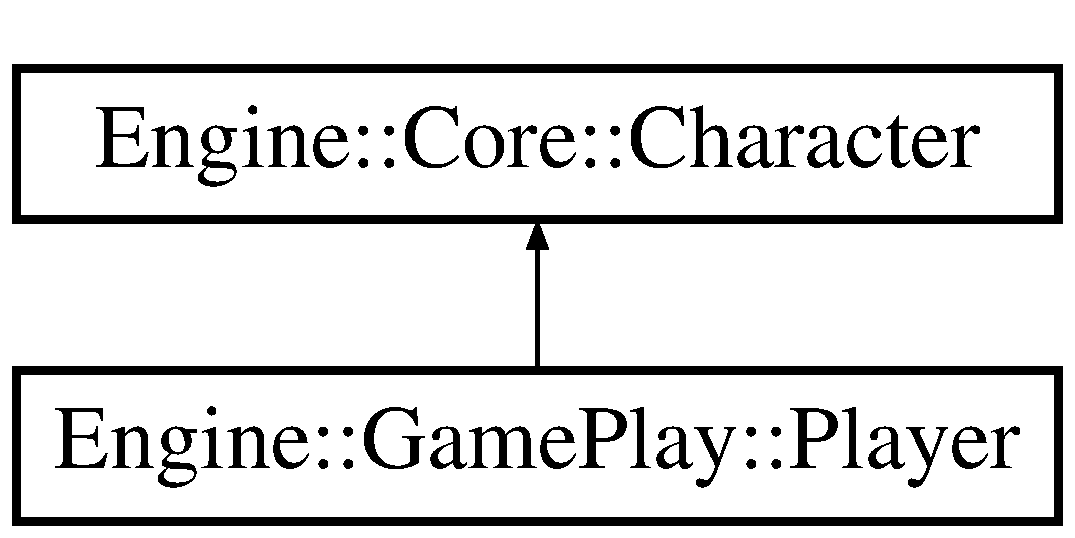
\includegraphics[height=2.000000cm]{class_engine_1_1_game_play_1_1_player}
\end{center}
\end{figure}
\subsection*{Public Member Functions}
\begin{DoxyCompactItemize}
\item 
\hyperlink{class_engine_1_1_game_play_1_1_player_a39c82fa94afe71949a7fff50fed2a4d0}{$\sim$\+Player} ()
\item 
void \hyperlink{class_engine_1_1_game_play_1_1_player_a06c682bf13c20fb2390807ec681b0121}{Update} (Render\+Window $\ast$Window, \hyperlink{class_engine_1_1_core_1_1_map}{Map} M, float dt) override
\item 
void \hyperlink{class_engine_1_1_game_play_1_1_player_adedc5552f70e5495ca1391b6f6143bec}{Set\+Enemy\+Manager} (void $\ast$Manager)
\item 
void \hyperlink{class_engine_1_1_game_play_1_1_player_a426ebc69b0607902e73563655ad66693}{Set\+Full\+Health} (void)
\item 
void \hyperlink{class_engine_1_1_game_play_1_1_player_aad2c7f9e75ef259e202be0d00924ec1d}{Regen\+Half\+Missing\+Health} (void)
\item 
void \hyperlink{class_engine_1_1_game_play_1_1_player_a4b3e08479cfc81c66eadf1e9da4a47fe}{Draw\+UI} (Render\+Window $\ast$Window)
\item 
\mbox{\Hypertarget{class_engine_1_1_game_play_1_1_player_a3705c78e4c21631432c4c21a0a4e4084}\label{class_engine_1_1_game_play_1_1_player_a3705c78e4c21631432c4c21a0a4e4084}} 
void {\bfseries Draw\+Weapon} (Render\+Window $\ast$Window)
\item 
shared\+\_\+ptr$<$ \hyperlink{class_engine_1_1_core_1_1_game_texture}{Game\+Texture} $>$ \hyperlink{class_engine_1_1_game_play_1_1_player_a22261e9c06350f20de748418085dd26a}{Get\+Player\+Weapon} (void) const
\end{DoxyCompactItemize}
\subsection*{Protected Member Functions}
\begin{DoxyCompactItemize}
\item 
\mbox{\Hypertarget{class_engine_1_1_game_play_1_1_player_a1ed8e67b1e585015f13614277470a188}\label{class_engine_1_1_game_play_1_1_player_a1ed8e67b1e585015f13614277470a188}} 
void {\bfseries Update\+UI} (void)
\end{DoxyCompactItemize}
\subsection*{Additional Inherited Members}


\subsection{Constructor \& Destructor Documentation}
\mbox{\Hypertarget{class_engine_1_1_game_play_1_1_player_a39c82fa94afe71949a7fff50fed2a4d0}\label{class_engine_1_1_game_play_1_1_player_a39c82fa94afe71949a7fff50fed2a4d0}} 
\index{Engine\+::\+Game\+Play\+::\+Player@{Engine\+::\+Game\+Play\+::\+Player}!````~Player@{$\sim$\+Player}}
\index{````~Player@{$\sim$\+Player}!Engine\+::\+Game\+Play\+::\+Player@{Engine\+::\+Game\+Play\+::\+Player}}
\subsubsection{\texorpdfstring{$\sim$\+Player()}{~Player()}}
{\footnotesize\ttfamily Engine\+::\+Game\+Play\+::\+Player\+::$\sim$\+Player (\begin{DoxyParamCaption}{ }\end{DoxyParamCaption})}

summary$>$ Updates the player and its status once per frame. /summary$>$ param name = \char`\"{}\+Window\char`\"{}$>$A pointer to the Render\+Window which is being used.

param name = \char`\"{}\+M\char`\"{}$>$A copy of the Map for the player for movement.

param name = \char`\"{}dt\char`\"{}$>$Delta time, the time the last frame took.

\subsection{Member Function Documentation}
\mbox{\Hypertarget{class_engine_1_1_game_play_1_1_player_a4b3e08479cfc81c66eadf1e9da4a47fe}\label{class_engine_1_1_game_play_1_1_player_a4b3e08479cfc81c66eadf1e9da4a47fe}} 
\index{Engine\+::\+Game\+Play\+::\+Player@{Engine\+::\+Game\+Play\+::\+Player}!Draw\+UI@{Draw\+UI}}
\index{Draw\+UI@{Draw\+UI}!Engine\+::\+Game\+Play\+::\+Player@{Engine\+::\+Game\+Play\+::\+Player}}
\subsubsection{\texorpdfstring{Draw\+U\+I()}{DrawUI()}}
{\footnotesize\ttfamily void Engine\+::\+Game\+Play\+::\+Player\+::\+Draw\+UI (\begin{DoxyParamCaption}\item[{Render\+Window $\ast$}]{Window }\end{DoxyParamCaption})}

summary$>$ Renders the weapon to the screen. /summary$>$ param name = \char`\"{}\+Window\char`\"{}$>$A pointer to the Render\+Window to draw to.\mbox{\Hypertarget{class_engine_1_1_game_play_1_1_player_a22261e9c06350f20de748418085dd26a}\label{class_engine_1_1_game_play_1_1_player_a22261e9c06350f20de748418085dd26a}} 
\index{Engine\+::\+Game\+Play\+::\+Player@{Engine\+::\+Game\+Play\+::\+Player}!Get\+Player\+Weapon@{Get\+Player\+Weapon}}
\index{Get\+Player\+Weapon@{Get\+Player\+Weapon}!Engine\+::\+Game\+Play\+::\+Player@{Engine\+::\+Game\+Play\+::\+Player}}
\subsubsection{\texorpdfstring{Get\+Player\+Weapon()}{GetPlayerWeapon()}}
{\footnotesize\ttfamily shared\+\_\+ptr$<$ \hyperlink{class_engine_1_1_core_1_1_game_texture}{Game\+Texture} $>$ Engine\+::\+Game\+Play\+::\+Player\+::\+Get\+Player\+Weapon (\begin{DoxyParamCaption}\item[{void}]{ }\end{DoxyParamCaption}) const}

summary$>$ Update the on screen UI. /summary$>$ \mbox{\Hypertarget{class_engine_1_1_game_play_1_1_player_aad2c7f9e75ef259e202be0d00924ec1d}\label{class_engine_1_1_game_play_1_1_player_aad2c7f9e75ef259e202be0d00924ec1d}} 
\index{Engine\+::\+Game\+Play\+::\+Player@{Engine\+::\+Game\+Play\+::\+Player}!Regen\+Half\+Missing\+Health@{Regen\+Half\+Missing\+Health}}
\index{Regen\+Half\+Missing\+Health@{Regen\+Half\+Missing\+Health}!Engine\+::\+Game\+Play\+::\+Player@{Engine\+::\+Game\+Play\+::\+Player}}
\subsubsection{\texorpdfstring{Regen\+Half\+Missing\+Health()}{RegenHalfMissingHealth()}}
{\footnotesize\ttfamily void Engine\+::\+Game\+Play\+::\+Player\+::\+Regen\+Half\+Missing\+Health (\begin{DoxyParamCaption}\item[{void}]{ }\end{DoxyParamCaption})}

summary$>$ Renders the UI to the screen. /summary$>$ param name = \char`\"{}\+Window\char`\"{}$>$A pointer to the Render\+Window to draw to.\mbox{\Hypertarget{class_engine_1_1_game_play_1_1_player_adedc5552f70e5495ca1391b6f6143bec}\label{class_engine_1_1_game_play_1_1_player_adedc5552f70e5495ca1391b6f6143bec}} 
\index{Engine\+::\+Game\+Play\+::\+Player@{Engine\+::\+Game\+Play\+::\+Player}!Set\+Enemy\+Manager@{Set\+Enemy\+Manager}}
\index{Set\+Enemy\+Manager@{Set\+Enemy\+Manager}!Engine\+::\+Game\+Play\+::\+Player@{Engine\+::\+Game\+Play\+::\+Player}}
\subsubsection{\texorpdfstring{Set\+Enemy\+Manager()}{SetEnemyManager()}}
{\footnotesize\ttfamily void Engine\+::\+Game\+Play\+::\+Player\+::\+Set\+Enemy\+Manager (\begin{DoxyParamCaption}\item[{void $\ast$}]{Manager }\end{DoxyParamCaption})}

summary$>$ Resets the health of the player to full. /summary$>$ \mbox{\Hypertarget{class_engine_1_1_game_play_1_1_player_a426ebc69b0607902e73563655ad66693}\label{class_engine_1_1_game_play_1_1_player_a426ebc69b0607902e73563655ad66693}} 
\index{Engine\+::\+Game\+Play\+::\+Player@{Engine\+::\+Game\+Play\+::\+Player}!Set\+Full\+Health@{Set\+Full\+Health}}
\index{Set\+Full\+Health@{Set\+Full\+Health}!Engine\+::\+Game\+Play\+::\+Player@{Engine\+::\+Game\+Play\+::\+Player}}
\subsubsection{\texorpdfstring{Set\+Full\+Health()}{SetFullHealth()}}
{\footnotesize\ttfamily void Engine\+::\+Game\+Play\+::\+Player\+::\+Set\+Full\+Health (\begin{DoxyParamCaption}\item[{void}]{ }\end{DoxyParamCaption})}

summary$>$ Sets the health of the player to half of the difference between the current amount of health and P\+L\+A\+Y\+E\+R\+\_\+\+M\+A\+X\+\_\+\+H\+E\+A\+L\+TH. /summary$>$ \mbox{\Hypertarget{class_engine_1_1_game_play_1_1_player_a06c682bf13c20fb2390807ec681b0121}\label{class_engine_1_1_game_play_1_1_player_a06c682bf13c20fb2390807ec681b0121}} 
\index{Engine\+::\+Game\+Play\+::\+Player@{Engine\+::\+Game\+Play\+::\+Player}!Update@{Update}}
\index{Update@{Update}!Engine\+::\+Game\+Play\+::\+Player@{Engine\+::\+Game\+Play\+::\+Player}}
\subsubsection{\texorpdfstring{Update()}{Update()}}
{\footnotesize\ttfamily void Engine\+::\+Game\+Play\+::\+Player\+::\+Update (\begin{DoxyParamCaption}\item[{Render\+Window $\ast$}]{Window,  }\item[{\hyperlink{class_engine_1_1_core_1_1_map}{Map}}]{M,  }\item[{float}]{dt }\end{DoxyParamCaption})\hspace{0.3cm}{\ttfamily [override]}, {\ttfamily [virtual]}}

summary$>$ Gets the enemies which in range of the player and then deals a random amount of damage, between 0 and P\+L\+A\+Y\+E\+R\+\_\+\+M\+A\+X\+\_\+\+A\+T\+T\+A\+C\+K\+\_\+\+D\+A\+M\+A\+GE. /summary$>$ 

Implements \hyperlink{class_engine_1_1_core_1_1_character}{Engine\+::\+Core\+::\+Character}.



The documentation for this class was generated from the following files\+:\begin{DoxyCompactItemize}
\item 
Wave\+Game/Player.\+h\item 
Wave\+Game/Player.\+cpp\end{DoxyCompactItemize}

\hypertarget{class_engine_1_1_core_1_1_texture_cache}{}\section{Engine\+:\+:Core\+:\+:Texture\+Cache Class Reference}
\label{class_engine_1_1_core_1_1_texture_cache}\index{Engine\+::\+Core\+::\+Texture\+Cache@{Engine\+::\+Core\+::\+Texture\+Cache}}
\subsection*{Static Public Attributes}
\begin{DoxyCompactItemize}
\item 
\mbox{\Hypertarget{class_engine_1_1_core_1_1_texture_cache_aaf8f2890aeb5dcb04dd3727a287965c9}\label{class_engine_1_1_core_1_1_texture_cache_aaf8f2890aeb5dcb04dd3727a287965c9}} 
static \hyperlink{class_engine_1_1_core_1_1_cache}{Cache}$<$ \hyperlink{class_engine_1_1_core_1_1_game_texture}{Game\+Texture} $>$ {\bfseries Cache} = \hyperlink{class_engine_1_1_core_1_1_cache}{Engine\+::\+Core\+::\+Cache}$<$\hyperlink{class_engine_1_1_core_1_1_game_texture}{Engine\+::\+Core\+::\+Game\+Texture}$>$()
\end{DoxyCompactItemize}


The documentation for this class was generated from the following files\+:\begin{DoxyCompactItemize}
\item 
Wave\+Game/Game\+Texture.\+h\item 
Wave\+Game/Game\+Texture.\+cpp\end{DoxyCompactItemize}

%--- End generated contents ---

% Index
\backmatter
\newpage
\phantomsection
\clearemptydoublepage
\addcontentsline{toc}{chapter}{Index}
\printindex

\end{document}
